% \begin{lemma}
%     \label{antipattern:lem:leq_gamma_mono_x_l}
%     \ \newline
%     \noindent
%     \begin{minipage}{0.7\textwidth}\setlength{\parindent}{1em}
%     Let $\mathcal{X} \mathop{=} (X, f:X \rightarrowtail F)$ be a ruler-graph and \( \rho \mathop{=} (L \overset{l}{\leftarrowtail} K \overset{r}{\rightarrowtail} R) \) be a rule. Consider the DPO diagram illustrated on the right. 
% \end{minipage}%
% \begin{minipage}{0.29\textwidth}
%     \hfill
%     \begin{tikzpicture}
%         % [node distance=15mm]
%         \node (I) {$K$};
%         \node (L) [left of=I] {$L$};
%         \node (R) [right of=I] {$R$};
%         \node (G) [below of=L] {$G$};
%         \node (C) [below of=I] {$C$};
%         \node (H) [below of=R] {$H$}; 
%         \draw [>->] (I) to  node [midway,below] {$l$} (L);
%         \draw [>->] (I) to  node [midway,below] {$r$} (R);
%         \draw [>->] (L) to node [midway,right] {$m$} (G);
%         \draw [>->] (I) to  node [midway,right] {$u$} (C); 
%         \draw [>->] (R) to  node [midway,right] {$m'$} (H);
%         \draw [>->] (C) to node [midway,above] {$l'$} (G);
%         \draw [>->] (C) to node [midway,above] {$r'$} (H);
%         % \node [at=($(I)!.5!(G)$)] {\normalfont PO};
%         % \node [at=($(I)!.5!(H)$)] {\normalfont PO};
%       \end{tikzpicture}
% \end{minipage} 

% We have
%         $  \{
%              h_{XL} \mathop{\in} \operatorname{Mono}(\mathcal{X},L)_{\operatorname{NF}} \mathop{\mid} 
%              \exists h_{FG}. h_{XL} \mathop{\star} m \mathop{=} f \mathop{\star} h_{FG}
%          \}
%          \mathop{\subseteq}
%             \Gamma(\operatorname{Mono}(\mathcal{X},L)_{\operatorname{NF}})
%             $ 
% \end{lemma}
% \begin{proof}


% \todo{useful?}

%     By Definition~\ref{antipattern:def:gamma_l_rho_x} of $\Gamma$.
% \end{proof}

\begin{lemma}
    \label{antipattern:lem:xgm_xhmp_xl_xr_llsss}
    Let $\mathcal{X} \mathop{=} (X, \set{f:X \rightarrowtail F})$ be a ruler-graph and \( \rho \mathop{=} (L \overset{l}{\leftarrowtail} K \overset{r}{\rightarrowtail} R) \) be a rule. Consider the DPO diagram:
   \begin{center}
        % \resizebox{0.5\textwidth}{!}{
   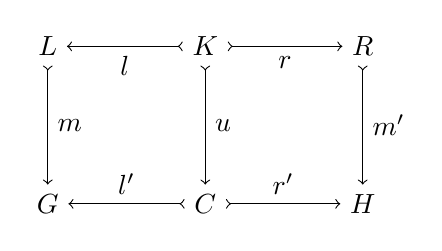
\begin{tikzpicture}
            % [node distance=15mm]
            \node (I) at (0,0) {$K$};
            \node (L)  at (-2,0) {$L$};
            \node (R)  at (2,0) {$R$};
            \node (G)  at (-2,-2) {$G$};
            \node (C)  at (0,-2) {$C$};
            \node (H)  at (2,-2) {$H$};
            \draw [>->] (I) to  node [midway,below] {$l$} (L);
            \draw [>->] (I) to  node [midway,below] {$r$} (R);
            \draw [>->] (L) to node [midway,right] {$m$} (G);
            \draw [>->] (I) to  node [midway,right] {$u$} (C);
            \draw [>->] (R) to  node [midway,right] {$m'$} (H);
            \draw [>->] (C) to node [midway,above] {$l'$} (G);
            \draw [>->] (C) to node [midway,above] {$r'$} (H);
            % \node [at=($(I)!.5!(G)$)] {\normalfont PO};
            % \node [at=($(I)!.5!(H)$)] {\normalfont PO};
        \end{tikzpicture}
        % }
    \end{center}

We have the following equalities:
\begin{flalign*}
    \card{\operatorname{Mono}(\mathcal{X},G,m)_{\operatorname{NF}}} \mathop{=} 
    &\card{\operatorname{Mono}(\mathcal{X},L)_{\operatorname{NF}}} - 
    \\
    &\card{\{
                h_{XL} \mathop{\in} \operatorname{Mono}(\mathcal{X},L)_{\operatorname{NF}} \mathop{\mid} 
                \exists h_{FG}. h_{XL} \mathop{\star} m \mathop{=} f \mathop{\star} h_{FG}
            \}},
    \\
    \card{\operatorname{Mono}(\mathcal{X},H,m')_{\operatorname{NF}}} \mathop{=} 
    &\card{\operatorname{Mono}(\mathcal{X},R)_{\operatorname{NF}}} - 
    \\
    &\card{\{
                h_{XR} \mathop{\in} \operatorname{Mono}(\mathcal{X},R)_{\operatorname{NF}} \mathop{\mid} 
                \exists h_{FH}. h_{XR} \mathop{\star} m' \mathop{=} f \mathop{\star} h_{FH} 
                \}}.
\end{flalign*}
\end{lemma}
\begin{proof}
    By symmetry, it suffices to prove the first equality, and the second equality follows. To prove the first equality, we show that there is a bijection between $\operatorname{Mono}(\mathcal{X},L)_{\operatorname{NF}} \mathop{\setminus} \{
                h_{XL} \mathop{\in} \operatorname{Mono}(\mathcal{X},L)_{\operatorname{NF}} \mathop{\mid} 
                \exists h_{FG}. h_{XL} \mathop{\star} m \mathop{=} f \mathop{\star} h_{FG}
            \}$ and $\operatorname{Mono}(\mathcal{X},G,m)_{\operatorname{NF}}$.

    Let $h_{XG} \mathop{\in} \operatorname{Mono}(\mathcal{X},G,m)_{\operatorname{NF}}$. By definition, there is a monomorphism $h_{XL}$ from $X$ to $L$ such that $h_{XG} \mathop{=} h_{XL} \mathop{\star} m$ and there is no monomorphism $h_{FG}$ from $F$ to $G$ such that $f \mathop{\star} h_{FG} \mathop{=} h_{XG}$. We must show $h_{XL} \mathop{\in} \operatorname{Mono}(\mathcal{X},L)_{\operatorname{NF}}$ and there is no $h_{FG}:f \rightarrowtail G$ such that $h_{XL} \mathop{\star} m \mathop{=} f \mathop{\star} h_{FG}$. These can be visualized by the following commutative diagram where edges that cannot exist are in red and dashed:

    \begin{center}
        \begin{tikzpicture}
            \node (k) at (0,1) {K};
            \node (l) at (-2,1) {L};
            \node (c) at (0,-1) {C};
            \node (g) at (-2,-1) {G};
            \node (x) at (-4,-3) {X};
            \node (f) at (-2,-3) {F};
            \draw[<-<]  (l) -- (k) node [midway,below] {$l$};
            \draw[>->] (c) -- (g) node [midway, above] {$l'$};
            \draw[>->] (l) -- (g) node[midway, right] {$m$};
            \draw[>->] (k) -- (c) node[midway, left] {};
            \draw[>->] (x) -- (g) node[midway,below] { };
            \draw[red,dashed,>->] (f) -- (g) node[midway] {$\times$};
            \draw[>->] (x) -- (l) node[midway,left] { };
            \draw[>->] (x) -- (f) node[midway,below] {$f$};
            \node () [at=($(l)!0.5!(c)$)] {$PO$};
        \end{tikzpicture}
    \end{center}
    
    We show $h_{XL} \mathop{\in} \operatorname{Mono}(\mathcal{X},L)_{\operatorname{NF}}$ by contradiction. Suppose that the contrary holds. There is a morphism $h_{FL}: F \rightarrowtail L$ such that $f \mathop{\star} h_{FL} \mathop{=} h_{XL}$.
    The image of $h_{XG}$ is, therefore, included in the image of $h_{FL} \mathop{\star} m$, as shown in the commutative diagram below, which contradicts the assumption that $h_{XG}$ is in $\operatorname{Mono}(\mathcal{X},G,m)_{\operatorname{NF}}$. 

    \begin{center}
        \begin{tikzpicture}
            \node (k) at (0,1) {K};
            \node (l) at (-2,1) {L};
            \node (c) at (0,-1) {C};
            \node (g) at (-2,-1) {G};
            \node (x) at (-4,-3) {X};
            \node (f) at (-4,-1) {F};
            \draw[<-<]  (l) -- (k) node [midway,below] {$l$};
            \draw[>->] (c) -- (g) node [midway, above] {$l'$};
            \draw[>->] (l) -- (g) node[midway, right] {$m$};
            \draw[>->] (k) -- (c) node[midway, left] {};
            \draw[>->] (x) -- (g) node[midway,below] { };
            \draw[>->] (f) -- (l) node[midway] {};
            \draw[>->] (x) -- (l) node[midway,left] { };
            \draw[>->] (x) -- (f) node[midway,left] {$f$};
            \node () [at=($(l)!0.5!(c)$)] {$PO$};
        \end{tikzpicture}
    \end{center}

    
    We show that there is no $h_{FG}:f \rightarrowtail G$ such that $h_{XL} \mathop{\star} m \mathop{=} f \mathop{\star} h_{FG}$ by contradiction. Suppose that the contrary holds. Under this assumption, we have the following commutative diagram. The image of $h_{XG}$ is, thus, included in the image of $f \mathop{\star} h_{FG}$ for some morphism $f$ which contradicts the assumption that $h_{XG}$ is in $\operatorname{Mono}(\mathcal{X},G,m)_{\operatorname{NF}}$.

    \begin{center}
        \begin{tikzpicture}
            \node (k) at (0,1) {K};
            \node (l) at (-2,1) {L};
            \node (c) at (0,-1) {C};
            \node (g) at (-2,-1) {G};
            \node (x) at (-4,-3) {X};
            \node (f) at (-2,-3) {F};
            \draw[<-<]  (l) -- (k) node [midway,below] {$l$};
            \draw[>->] (c) -- (g) node [midway, above] {$l'$};
            \draw[>->] (l) -- (g) node[midway, right] {$m$};
            \draw[>->] (k) -- (c) node[midway, left] {};
            \draw[>->] (x) -- (g) node[midway,below] { };
            \draw[>->] (f) -- (g) node[midway,right] {};
            \draw[>->] (x) -- (l) node[midway,left] { };
            \draw[>->] (x) -- (f) node[midway,below] {$f$};
            \node () [at=($(l)!0.5!(c)$)] {$PO$};
        \end{tikzpicture}
    \end{center}

    Let $h_{XG}, h_{XG}' \mathop{\in} \operatorname{Mono}(\mathcal{X},G,m)_{\operatorname{NF}}$ such that $h_{XG} \mathop{\neq} h_{XG}'$. By definition, there are morphisms $h_{XL}, h_{XL}': X \rightarrowtail L$ such that $h_{XG} \mathop{=} h_{XL} \mathop{\star} m$, $h_{XG}' \mathop{=} h_{XL}' \mathop{\star} m$, and no morphism $h_{FG}, h_{FG}': F \rightarrowtail G$ such that $f \mathop{\star} h_{FG} \mathop{=} h_{XG}$ and $f \mathop{\star} h_{FG}' \mathop{=} h_{XG}'$. Since $m$ is injection, we have $h_{XL} \mathop{\neq} h_{XL}'$.

    There is, therefore, an injection from the set $\operatorname{Mono}(\mathcal{X},G,m)_{\operatorname{NF}}$ to the set $\operatorname{Mono}(\mathcal{X},L)_{\operatorname{NF}} \mathop{\setminus} \{
                h_{XL} \mathop{\in} \operatorname{Mono}(\mathcal{X},L)_{\operatorname{NF}} \mathop{\mid} 
                \exists h_{FG}. h_{XL} \mathop{\star} m \mathop{=} f \mathop{\star} h_{FG}
            \}$.

    Conversely, let $h_{XL}$ be a morphism of the following set $$\operatorname{Mono}(\mathcal{X},L)_{\operatorname{NF}}\mathop{\setminus} \{
                h_{XL} \mathop{\in} \operatorname{Mono}(\mathcal{X},L)_{\operatorname{NF}} \mathop{\mid} 
                \exists h_{FG}. h_{XL} \mathop{\star} m \mathop{=} f \mathop{\star} h_{FG}
            \}.$$ 
    We have the following commutative diagram:
    
    \begin{center}
        \begin{tikzpicture}
            \node (k) at (0,1) {K};
            \node (l) at (-2,1) {L};
            \node (c) at (0,-1) {C};
            \node (g) at (-2,-1) {G};
            \node (x) at (-4,-3) {X};
            \node (f) at (-4,-1) {F};
            \draw[<-<]  (l) -- (k) node [midway,below] {$l$};
            \draw[>->] (c) -- (g) node [midway, above] {$l'$};
            \draw[>->] (l) -- (g) node[midway, right] {$m$};
            \draw[>->] (k) -- (c) node[midway, left] {};
            \draw[red,dashed,>->] (f) -- (l) node[midway] {$\times$};
            \draw[>->] (x) -- (l) node[midway,left] { };
            \draw[>->] (x) -- (f) node[midway,left] {$f$};
            \draw[red,dashed,>->] (f) -- (g) node[pos=0.75] {$\times$};
            \node () [at=($(l)!0.5!(c)$)] {$PO$};
        \end{tikzpicture}
    \end{center}
    To prove $h_{XL} \mathop{\star} m \mathop{\in} \operatorname{Mono}(\mathcal{X},G,m)_{\operatorname{NF}}$, we show that $h_{XL} \mathop{\star} m$ is an element of $\operatorname{Mono}(\mathcal{X},G,m)$ and that there is no morphism $h_{FG}: F \rightarrowtail G$ such that $f \mathop{\star} h_{FG} \mathop{=} h_{XL} \mathop{\star} m$. We have $h_{XL} \mathop{\star} m \mathop{\in} \operatorname{Mono}(\mathcal{X},G,m)$, because the equality $h_{XL} \mathop{\star} m \mathop{=} f \mathop{\star} h_{FG}$ holds by definition. There is no morphism $h_{FG}: F \rightarrowtail G$ such that $f \mathop{\star} h_{FG} \mathop{=} h_{XL} \mathop{\star} m$, by definition of $h_{XL}$.

    Let $h_{XL}, h_{XL}'$ be morphisms in the following set
     $$\operatorname{Mono}(\mathcal{X},L)_{\operatorname{NF}}\mathop{\setminus} \{
                h_{XL} \mathop{\in} \operatorname{Mono}(\mathcal{X},L)_{\operatorname{NF}} \mathop{\mid} 
                \exists h_{FG}. h_{XL} \mathop{\star} m \mathop{=} f \mathop{\star} h_{FG}
    \}$$
    such that $h_{XL} \mathop{\neq} h_{XL}'$.
    Since $m$ is injective, we have $h_{XL} \mathop{\star} m \mathop{\neq} h_{XL}' \mathop{\star} m$. 
 
    There is, thus, an injection from the following set
 $$  (\operatorname{Mono}(\mathcal{X},L)_{\operatorname{NF}}\mathop{\setminus} \{
                h_{XL} \mathop{\in} \operatorname{Mono}(\mathcal{X},L)_{\operatorname{NF}} \mathop{\mid} 
                \exists h_{FG}. h_{XL} \mathop{\star} m \mathop{=} f \mathop{\star} h_{FG}
            \}) \mathop{\star} m$$
    to $\operatorname{Mono}(\mathcal{X},G,m)_{\operatorname{NF}}$.
    Since the following two sets are in bijection
    \begin{itemize}
        \item $(\operatorname{Mono}(\mathcal{X},L)_{\operatorname{NF}}\mathop{\setminus} \{
                h_{XL} \mathop{\in} \operatorname{Mono}(\mathcal{X},L)_{\operatorname{NF}} \mathop{\mid} 
                \exists h_{FG}. h_{XL} \mathop{\star} m \mathop{=} f \mathop{\star} h_{FG}
            \}) \mathop{\star} m$, 
        \item $\operatorname{Mono}(\mathcal{X},L)_{\operatorname{NF}}\mathop{\setminus} \{
                h_{XL} \mathop{\in} \operatorname{Mono}(\mathcal{X},L)_{\operatorname{NF}} \mathop{\mid} 
                \exists h_{FG}. h_{XL} \mathop{\star} m \mathop{=} f \mathop{\star} h_{FG}
            \}$,
    \end{itemize} 
    we conclude that there is an injection from the set $A$ to $\operatorname{Mono}(\mathcal{X},G,m)_{\operatorname{NF}}$, where $A \isdef \operatorname{Mono}(\mathcal{X},L)_{\operatorname{NF}}\mathop{\setminus} \{
                h_{XL} \mathop{\in} \operatorname{Mono}(\mathcal{X},L)_{\operatorname{NF}} \mathop{\mid} 
                \exists h_{FG}. h_{XL} \mathop{\star} m \mathop{=} f \mathop{\star} h_{FG}
            \}$.

    Finally, we conclude.
\end{proof}



\noindent
\begin*{\textbf{Lemma~\ref{antipattern:lem:xgm_xhmp_xl_xr}}}
%     \newline
%     \noindent
% \begin{minipage}{0.7\textwidth}\setlength{\parindent}{1em}
%     Let $\mathcal{X}=(X,\mathcal{C})$
%     % $\mathcal{X} \mathop{=} (X, f:X \rightarrowtail F)$
%      be a ruler-graph and \( \rho \mathop{=} (L \overset{l}{\leftarrowtail} K \overset{r}{\rightarrowtail} R) \) be a rule. Consider the DPO diagram illustrated on the right. 
% \end{minipage}%
% \begin{minipage}{0.29\textwidth}
%     \hfill
%     \begin{tikzpicture}
%         % [node distance=15mm]
%         \node (I) {$K$};
%         \node (L) [left of=I] {$L$};
%         \node (R) [right of=I] {$R$};
%         \node (G) [below of=L] {$G$};
%         \node (C) [below of=I] {$C$};
%         \node (H) [below of=R] {$H$}; 
%         \draw [>->] (I) to  node [midway,below] {$l$} (L);
%         \draw [>->] (I) to  node [midway,below] {$r$} (R);
%         \draw [>->] (L) to node [midway,right] {$m$} (G);
%         \draw [>->] (I) to  node [midway,right] {$u$} (C); 
%         \draw [>->] (R) to  node [midway,right] {$m'$} (H);
%         \draw [>->] (C) to node [midway,above] {$l'$} (G);
%         \draw [>->] (C) to node [midway,above] {$r'$} (H);
%         % \node [at=($(I)!.5!(G)$)] {\normalfont PO};
%         % \node [at=($(I)!.5!(H)$)] {\normalfont PO};
%       \end{tikzpicture}
% \end{minipage} 

% We have 
%     $$
%         \card{\operatorname{Mono}(\mathcal{X},G,m)_{\operatorname{NF}}} - 
%         \card{\operatorname{Mono}(\mathcal{X},H,m')_{\operatorname{NF}}} \geq
%         \Lambda(\mathcal{X}, \rho)
%     $$
%     where $\Lambda(\mathcal{X},\rho) \overset{\operatorname{def}}{=} \card{\operatorname{Mono}(\mathcal{X},L)_{\operatorname{NF}}} - 
%     \card{\Gamma(\operatorname{Mono}(\mathcal{X},L)_{\operatorname{NF}})} -
%    \card{\operatorname{Mono}(\mathcal{X},R)_{\operatorname{NF}}}$.

  Let $\mathcal{X} \mathop{=} (X, \set{f:X \rightarrowtail F})$ be a ruler-graph, and let \( \rho \mathop{=} (L \overset{l}{\leftarrowtail} K \overset{r}{\rightarrowtail} R) \) be a rule. 
  Consider the DPO diagram shown below.

   \begin{center}
        % \resizebox{0.5\textwidth}{!}{
   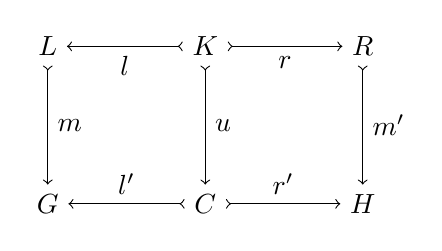
\begin{tikzpicture}
            % [node distance=15mm]
            \node (I) at (0,0) {$K$};
            \node (L)  at (-2,0) {$L$};
            \node (R)  at (2,0) {$R$};
            \node (G)  at (-2,-2) {$G$};
            \node (C)  at (0,-2) {$C$};
            \node (H)  at (2,-2) {$H$};
            \draw [>->] (I) to  node [midway,below] {$l$} (L);
            \draw [>->] (I) to  node [midway,below] {$r$} (R);
            \draw [>->] (L) to node [midway,right] {$m$} (G);
            \draw [>->] (I) to  node [midway,right] {$u$} (C);
            \draw [>->] (R) to  node [midway,right] {$m'$} (H);
            \draw [>->] (C) to node [midway,above] {$l'$} (G);
            \draw [>->] (C) to node [midway,above] {$r'$} (H);
            % \node [at=($(I)!.5!(G)$)] {\normalfont PO};
            % \node [at=($(I)!.5!(H)$)] {\normalfont PO};
        \end{tikzpicture}
        % }
    \end{center}

We have 
    $$
        \card{\operatorname{Mono}(\mathcal{X},G,m)_{\operatorname{NF}}} - 
        \card{\operatorname{Mono}(\mathcal{X},H,m')_{\operatorname{NF}}} \geq
        \Lambda(\mathcal{X}, \rho)
    $$
    where $\Lambda(\mathcal{X},\rho) \overset{\operatorname{def}}{=} \card{\operatorname{Mono}(\mathcal{X},L)_{\operatorname{NF}}} - 
    \card{\Gamma(\operatorname{Mono}(\mathcal{X},L)_{\operatorname{NF}})} -
   \card{\operatorname{Mono}(\mathcal{X},R)_{\operatorname{NF}}}$.
\end*{}

\begin{proof}
    \label{antipattern:proof:lem:xgm_xhmp_xl_xr}
    There are two cases to consider: either $\mathcal{C}=\emptyset$ or $\mathcal{C}=\set{f:X \rightarrowtail F}$. For the first case, since $\Gamma(\operatorname{Mono}(\mathcal{X},L)_{\operatorname{NF}}) \mathop{=} \emptyset$ by definition, the inequality is equivalent to the following:
    $$
        \card{\operatorname{Mono}(\mathcal{X},G,m)_{\operatorname{NF}}} - 
        \card{\operatorname{Mono}(\mathcal{X},H,m')_{\operatorname{NF}}} \geq
        \card{\operatorname{Mono}(\mathcal{X},L)_{\operatorname{NF}}} - 
        \card{\operatorname{Mono}(\mathcal{X},R)_{\operatorname{NF}}}.
    $$
    By definition, it is equivalent to the inequality:
    \begin{flalign*}
        \card{\operatorname{Mono}(X,G,m)} - 
        \card{\operatorname{Mono}(X,H,m')} \mathop{\geq}  
        \card{\operatorname{Mono}(X,L)} - 
   \card{\operatorname{Mono}(X,R)}
    \end{flalign*}
    because the following equalities hold by Lemma~\ref{subgraph_counting:lem:decomp_w_u}:
    \begin{itemize}
        \item $\card{\operatorname{Mono}(X,G,m)} \mathop{=} \card{\operatorname{Mono}(X,L)}$,
        \item $\card{\operatorname{Mono}(X,H,m')} =
   \card{\operatorname{Mono}(X,R)}$.
    \end{itemize} 

   For the second case, by Lemma~\ref{antipattern:lem:xgm_xhmp_xl_xr_llsss}, we have the following:
    \begin{flalign*}
        &\card{\operatorname{Mono}(\mathcal{X},G,m)_{\operatorname{NF}}} - 
        \card{\operatorname{Mono}(\mathcal{X},H,m')_{\operatorname{NF}}} 
        \\
        \mathop{=} &(\card{\operatorname{Mono}(\mathcal{X},L)_{\operatorname{NF}}} - 
            \card{\{
                h_{XL} \mathop{\in} \operatorname{Mono}(\mathcal{X},L)_{\operatorname{NF}} \mathop{\mid} 
                \exists h_{FG}. h_{XL} \mathop{\star} m \mathop{=} f \mathop{\star} h_{FG}
            \}}
        ) - 
        \\
            &
           (
            \card{\operatorname{Mono}(\mathcal{X},R)_{\operatorname{NF}}}
            -  
            \card{\{
                h_{XR} \mathop{\in} \operatorname{Mono}(\mathcal{X},R)_{\operatorname{NF}} \mathop{\mid} 
                \exists h_{FH}. h_{XR} \mathop{\star} m' \mathop{=} f \mathop{\star} h_{FH}
            \}}
           )
    \end{flalign*}
    where 
    $\{
                h_{XL} \mathop{\in} \operatorname{Mono}(\mathcal{X},L)_{\operatorname{NF}} \mathop{\mid} 
                \exists h_{FG}. h_{XL} \mathop{\star} m \mathop{=} h_{XF} \mathop{\star} h_{FG}
            \}$ is the set of occurrences of $X$ in $L$ that are not included in any occurrences of its forbidden context in $L$ but included in an occurrence of its forbidden context in $G$, and, analogously, $\{
                h_{XR} \mathop{\in} \operatorname{Mono}(\mathcal{X},R)_{\operatorname{NF}} \mathop{\mid} 
                \exists h_{FH}. h_{XR} \mathop{\star} m' \mathop{=} h_{XF} \mathop{\star} h_{FH}
            \}$ is the set of $X$-occurrences in $R$ that are not included in any occurrences of its forbidden context in $R$ but included in an occurrence of its forbidden context in $H$.

    The following equalities and inequalities hold:
    \begin{flalign*}
        &\card{\operatorname{Mono}(\mathcal{X},G,m)_{\operatorname{NF}}} \mathop{-} 
        \card{\operatorname{Mono}(\mathcal{X},H,m')_{\operatorname{NF}}} 
        \\
           \mathop{=} &(\card{\operatorname{Mono}(\mathcal{X},L)_{\operatorname{NF}}} \mathop{-} 
           \card{\operatorname{Mono}(\mathcal{X},R)_{\operatorname{NF}}}
       )\mathop{+}
       \\
           &
          (
            \card{\{
               h_{XR} \mathop{\in} \operatorname{Mono}(\mathcal{X},R)_{\operatorname{NF}} \mathop{\mid} 
               \exists h_{FH}. h_{XR} \mathop{\star} m' \mathop{=} f \mathop{\star} h_{FH}
           \}}
           \mathop{-} \\&
           \card{\{
                h_{XL} \mathop{\in} \operatorname{Mono}(\mathcal{X},L)_{\operatorname{NF}} \mathop{\mid} 
                \exists h_{FG}. h_{XL} \mathop{\star} m \mathop{=} f \mathop{\star} h_{FG}
            \}}         
          ) 
        \\ 
        \mathop{\geq}& (\card{\operatorname{Mono}(\mathcal{X},L)_{\operatorname{NF}}} \mathop{-} 
        \card{\operatorname{Mono}(\mathcal{X},R)_{\operatorname{NF}}}
        ) \mathop{-}
         \\
         & \card{\{
             h_{XL} \mathop{\in} \operatorname{Mono}(\mathcal{X},L)_{\operatorname{NF}} \mathop{\mid} 
             \exists h_{FG}. h_{XL} \mathop{\star} m \mathop{=} h_{XF} \mathop{\star} h_{FG}
         \}}        
       \\ 
       \mathop{=}& (\card{\operatorname{Mono}(\mathcal{X},L)_{\operatorname{NF}}} \mathop{-} 
       \card{\operatorname{Mono}(\mathcal{X},R)_{\operatorname{NF}}}
       ) \mathop{-} 
       \\
       &
    %   (
    %     0 \mathop{-}   
       \card{
        \Gamma(\operatorname{Mono}(\mathcal{X},L)_{\operatorname{NF}})
        }      
    %   )  
        & \text{by Definition~\ref{antipattern:def:gamma_l_rho_x}}
      \\
      \mathop{=}& 
      \card{\operatorname{Mono}(\mathcal{X},L)_{\operatorname{NF}}} \mathop{-} 
      \card{
        \Gamma(\operatorname{Mono}(\mathcal{X},L)_{\operatorname{NF}})
        } \mathop{-}
      \card{\operatorname{Mono}(\mathcal{X},R)_{\operatorname{NF}}}
      \\
      \mathop{=}& \Lambda(\mathcal{X}, \rho).
    \end{flalign*}
\end{proof}

\begin{lemma}
    \label{antipattern:lem:xh_decomp}
     Consider the following pushout diagram in the category \textbf{Graph}:
     \begin{center}
        \begin{tikzpicture}
            \node (k) at (0,1) {K};
            \node (r) at (2,1) {R};
            \node (c) at (0,-1) {C};
            \node (h) at (2,-1) {H};
            \draw[>->]  (k) -- (r) node [midway,below] {$r$};
            \draw[>->] (c) -- (h) node [midway,above] {$r'$};
            \draw[>->] (r) -- (h) node[midway, left] {$m'$};
            \draw[>->] (k) -- (c) node[midway, left] {};
            \node () [at=($(r)!0.5!(c)$)] {$PO$};
        \end{tikzpicture}
    \end{center}
    Let $X$ be a graph, and $h_{XH}:X \rightarrowtail H$ a monomorphism. Then, we can construct the following commutative diagram in the category \textbf{Graph}: 

    \begin{center}
        % \resizebox{0.3\textwidth}{!}{
            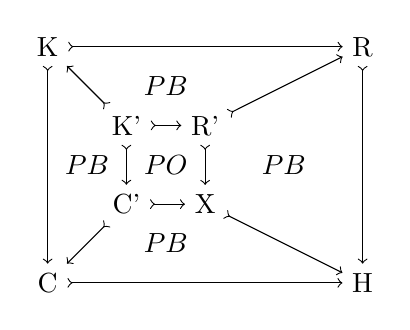
\begin{tikzpicture}
                \node (k) at (0,0) {K};
                \node (r) at (4,0) {R};
                \node (c) at (0,-3) {C};
                \node (h) at (4,-3) {H};
                \draw[<-<]  (r) -- (k) node [midway,above] {};
                \draw[>->] (c) -- (h) node [midway, below] {};
                \draw[>->] (r) -- (h) node[midway, left] {};
                \draw[>->] (k) -- (c) node[midway, left] {};
                \node (k') at (1,-1) {K'};
                \node (r') at (2,-1) {R'};
                \node (c') at (1,-2) {C'};
                \node () at (1.5,-1.5) {$PO$};
                \node () at (3,-1.5) {$PB$};
                \node () at (1.5,-2.5) {$PB$};
                \node () at (1.5,-0.5) {$PB$};
                \node () at (0.5,-1.5) {$PB$};
                \node (x) at (2,-2) {X};
                \draw [>->] (c') -- (x);
                \draw [>->] (r') -- (x);
                \draw [>->] (k') -- (r');
                \draw [>->] (k') -- (c');
                \draw [>->] (c') -- (c);
                \draw[>->] (r') -- (r);
                \draw[>->] (x) -- (h) node[midway,right] {};
                \draw[>->] (k') -- (k) ;
            \end{tikzpicture}
        % }
        \end{center} 
\end{lemma}
\begin{proof}    
         In the category \textbf{Graph}, we can construct the following commutative diagram \todo{should I give more details?}:
        \begin{center}
            % \resizebox{0.3\textwidth}{!}{
                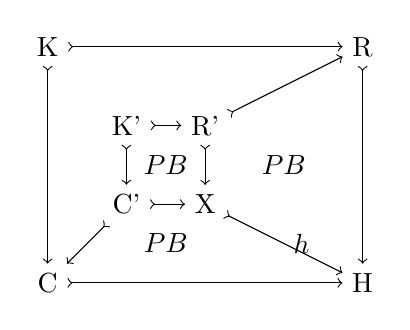
\begin{tikzpicture}
                    \node (k) at (0,0) {K};
                    \node (r) at (4,0) {R};
                    \node (c) at (0,-3) {C};
                    \node (h) at (4,-3) {H};
                    % \node (rb) at ($\scl*(1.5,-0.5)$) {$R_X$};
                    
                    % \node (h') at ($\scl*(1.5,-1.5)$) {$H'$};
                    % \draw[>->]  (rb) -- (h') node [midway,above] {};
                    % \draw[>->]  (c) -- (h') node [midway,above] {};
        
                    \draw[<-<]  (r) -- (k) node [midway,above] {};
                    \draw[>->] (c) -- (h) node [midway, below] {};
                    \draw[>->] (r) -- (h) node[midway, left] {};
                    \draw[>->] (k) -- (c) node[midway, left] {};
        
                    % \draw[->] (rb) to (l);
                    % \draw[<-<] (rb) to (k);
                
                    \node (k') at (1,-1) {K'};
                    \node (r') at (2,-1) {R'};
                    \node (c') at (1,-2) {C'};
                    \node () at (1.5,-1.5) {$PB$};
                    \node () at (3,-1.5) {$PB$};
                    \node () at (1.5,-2.5) {$PB$};
                    \node (x) at (2,-2) {X};
                    % \draw [->] (x) -- (h') node[midway] {!};
                    \draw [>->] (c') -- (x);
                    \draw [>->] (r') -- (x);
                    \draw [>->] (k') -- (r');
                    \draw [>->] (k') -- (c');
                    \draw [>->] (c') -- (c);
                    % \draw [->] (r') -- (rb);
                    % \draw [->] (r') -- (rb);
                    % \draw [->] (h') -- (h);
        
                    \draw[>->] (r') -- (r);
                    \draw[>->] (x) -- (h) node[midway,right] {$h$};
                    % \node (rb) at ($\scl*(\sclx*1.5,-0.5)$) {$R_X$};
                    % \node (h') at ($\scl*(\sclx*1.5,-1.2)$) {$H'$};
                    % \draw[>->]  (rb) -- (h') node [midway,above] {};
                    % \draw[>->]  (c) -- (h') node [midway,above] {};
                    % \draw[>->]  (rb) -- (h') node [midway,above] {};
                    % \draw[>->] (rb) to (r);
                    % \draw[<-<] (rb) to (k);
                \end{tikzpicture}
            % }
            \end{center} 
        
        Since $KCHR$ is a pushout, it is also a pullback, by Proposition~\ref{prop:pb_eq_po}. 
        Therefore, from \(
            h_{K'C'} \mathop{\star} h_{C'C} \mathop{\star} h_{CH} =h_{K'R'} \mathop{\star} h_{R'R} \mathop{\star} h_{R'R}
        \) and the universal property of pullback, there is a unique morphism $h_{K'K}:K' \rightarrowtail K$ such that 
        \begin{flalign*}
            h_{K'C'} \mathop{\star} h_{C'C} &= h_{K'K} \mathop{\star} h_{KC}, 
            % \label{antipattern:kpcpcpckpkkc}
            \\
            h_{K'R'} \mathop{\star} h_{R'R} &= h_{K'K} \mathop{\star} h_{KR}.
            % \label{antipattern:kprprprkpk}
         \end{flalign*}
        The square $K'KCC'$ and $K'R'RK$ are pullbacks, by Lemma~\ref{kpcpck_pullback}. Furthermore, $K'C'XR'$ is a pushout by Lemma~\ref{kpcpxrp_po}. Hence, the following commutative diagram holds:
        \begin{center}
                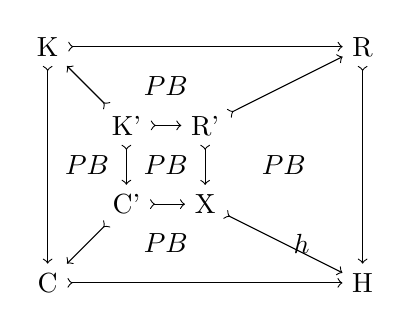
\begin{tikzpicture}
                    \node (k) at (0,0) {K};
                    \node (r) at (4,0) {R};
                    \node (c) at (0,-3) {C};
                    \node (h) at (4,-3) {H};
                    \draw[<-<]  (r) -- (k) node [midway,above] {};
                    \draw[>->] (c) -- (h) node [midway, below] {};
                    \draw[>->] (r) -- (h) node[midway, left] {};
                    \draw[>->] (k) -- (c) node[midway, left] {};
                    \node (k') at (1,-1) {K'};
                    \node (r') at (2,-1) {R'};
                    \node (c') at (1,-2) {C'};
                    \node () at (1.5,-1.5) {$PB$};
                    \node () at (3,-1.5) {$PB$};
                    \node () at (1.5,-2.5) {$PB$};
                    \node () at (1.5,-0.5) {$PB$};
                    \node () at (0.5,-1.5) {$PB$};
                    \node (x) at (2,-2) {X};
                    \draw [>->] (c') -- (x);
                    \draw [>->] (r') -- (x);
                    \draw [>->] (k') -- (r');
                    \draw [>->] (k') -- (c');
                    \draw [>->] (c') -- (c);
                    \draw[>->] (r') -- (r);
                    \draw[>->] (x) -- (h) node[midway,right] {$h$};
                    \draw[>->] (k') -- (k) ;
                \end{tikzpicture}
            \end{center} 
        \todo{use: assumption: non increasing}
\end{proof}

\noindent
\begin*{\textbf{Lemma~\ref{antipattern:lem:xglnotmlp_xhlnotmrp}}}
        Let \( \rho \mathop{=} (L \overset{l}{\leftarrowtail} K \overset{r}{\rightarrowtail} R) \) be a rule and $\mathcal{X}=(X,\mathcal{C})$ be a ruler-graph with underlying graph $X$.
        Suppose that $\rho^{-1}$ is $F$-non-increasing if $\mathcal{C} \mathop{=} \set{f:X \rightarrowtail F}$. For the DPO diagram:
        \begin{center}
            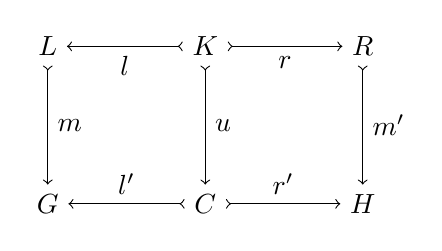
\begin{tikzpicture}
                \node (I) at (0,0) {$K$};
                \node (L) at (-2,0) {$L$};
                \node (R) at (2,0) {$R$};
                \node (G) at (-2,-2) {$G$}; 
                \node (C) at (0,-2) {$C$};
                \node (H) at (2,-2) {$H$}; 
                \draw [>->] (I) to  node [midway,below] {$l$} (L);
                \draw [>->] (I) to  node [midway,below] {$r$} (R);
                \draw [>->] (L) to node [midway,right] {$m$} (G);
                \draw [>->] (I) to  node [midway,right] {$u$} (C); 
                \draw [>->] (R) to  node [midway,right] {$m'$} (H);
                \draw [>->] (C) to node [midway,above] {$l'$} (G);
                \draw [>->] (C) to node [midway,above] {$r'$} (H);
             \end{tikzpicture}
        \end{center}
        the following inequality holds:
    $$\card{\operatorname{Mono}(\mathcal{X},G,\mathop{\lnot} m, l')_{\operatorname{NF}}} \geq
        \card{\operatorname{Mono}(\mathcal{X},H,\mathop{\lnot} m', r')_{\operatorname{NF}}}.$$
\end*{}
\begin{proof}
    \label{antipattern:proof:lem:xglnotmlp_xhlnotmrp}
    There are two cases to consider: either $\mathcal{C} \mathop{=}\emptyset$ or $\mathcal{C} \mathop{=} \set{f:X \rightarrowtail F}$. 
     In the first case, since there is no forbidden context, the inequality is equivalent to $
        \card{\operatorname{Mono}(\mathcal{X},G,\lnot m, l')} \geq
        \card{\operatorname{Mono}(\mathcal{X},H,\lnot m', r')}$.
    To show this inequality, we are going to establish an injection from $\operatorname{Mono}(\mathcal{X},H,\lnot m', r')$ to $\operatorname{Mono}(\mathcal{X},G,\lnot m, l')$. Let $h_{XH} \mathop{\in} \operatorname{Mono}(\mathcal{X},H,\lnot m', r')$. By definition, there is a monomorphism $h_{XC}:X \rightarrowtail C$ such that $h_{XH} \mathop{=} h_{XC} \mathop{\star} r'$. Thus we have the following commutative diagram:

     \begin{center}
        \begin{tikzpicture}
            \node (k) at (0,1) {K};
            \node (l) at (-2,1) {L};
            \node (r) at (2,1) {R};
            \node (c) at (0,-1) {C};
            \node (g) at (-2,-1) {G};
            \node (h) at (2,-1) {H};
            \node (x) at (4,-2) {X};
            \draw[>->] (x) -- (h) node [midway,above] {};
            \draw[>->] (x) edge (c) node [midway,above] {};
            \draw[>->]  (k) -- (r) node [midway,below] {$r$};
            \draw[>->]  (k) -- (l) node [midway,below] {$l$};
            \draw[>->] (c) -- (g) node [midway, above] {$l'$};
            \draw[>->] (c) -- (h) node [midway,above] {$r'$};
            \draw[>->] (l) -- (g) node[midway, right] {$m$};
            \draw[>->] (r) -- (h) node[midway, left] {$m'$};
            \draw[>->] (k) -- (c) node[midway, left] {$u$};
            \node () [at=($(l)!0.5!(c)$)] {$PO$};
            \node () [at=($(r)!0.5!(c)$)] {$PO$};
        \end{tikzpicture}
    \end{center}
    We must show $h_{XC} \mathop{\star} l' \mathop{\in} \operatorname{Mono}(\mathcal{X},G,\lnot m, l')$ which is equivalent to showing that there is no $h_{XL}$ such that 
    $h_{XL} \mathop{\star} m \mathop{=} h_{XC} \mathop{\star} l'$.
    Suppose that the contrary holds.
     Since $KLGC$ is a pullback by Proposition~\ref{prop:pb_eq_po}, there is a morphism $h_{XK}:X \rightarrowtail K$ such that 
            \begin{flalign}
         h_{XK} \mathop{\star} u \mathop{=} h_{XC}. \label{alabeldkfsjlk}
        \end{flalign} 
    Therefore, we have 
    \begin{flalign*}
        h_{XH} 
        &= h_{XC} \mathop{\star} r' \\
        &= (h_{XK} \mathop{\star} u) \mathop{\star} r' 
       & \text{by~\eqref{alabeldkfsjlk}}\\
        &= h_{XK} \mathop{\star} (r \mathop{\star} m') \\ 
        &= (h_{XK} \mathop{\star} r) \mathop{\star} m'.
    \end{flalign*}
    This contradicts the fact that $h_{XH} \mathop{\in} \operatorname{Mono}(\mathcal{X},H,\lnot m', r')$. Therefore, we have $h_{XC} \mathop{\star} l' \mathop{\in} \operatorname{Mono}(\mathcal{X},G,\lnot m, l')$.

    Furthermore, if $h_{XH}, h_{XH}' \mathop{\in} \operatorname{Mono}(\mathcal{X},H,\lnot m', r')$ with $h_{XH} \mathop{\neq} h_{XH}'$, then there are $h_{XC}, h_{XC}'$ such that $h_{XH} \mathop{=} h_{XC} \mathop{\star} r'$ and $h_{XH}' \mathop{=} h_{XC}' \mathop{\star} r'$. Since $r'$ is injective, we deduce that $h_{XC} \mathop{\neq} h_{XC}'$. Therefore, from the injectivity of $l'$, we have $h_{XC} \mathop{\star} l' \mathop{\neq} h_{XC}' \mathop{\star} l'$. Thus, there is an injection from $\operatorname{Mono}(\mathcal{X},H,\lnot m', r')$ to $\operatorname{Mono}(\mathcal{X},G,\lnot m, l')$, which proves the inequality.
        
        Now, let us focus on the second case, where $\mathcal{X} \mathop{=} (X, f:X \rightarrowtail F)$. We have the following equalities:
        \begin{flalign*}
            &\card{\operatorname{Mono}(\mathcal{X},G,\lnot m, l')_{\operatorname{NF}}} - 
            \card{\operatorname{Mono}(,H,\lnot m', r')_{\operatorname{NF}}} 
           \\
            \mathop{=} &(\card{\operatorname{Mono}(X,G,\lnot m, l')} - \card{\operatorname{Mono}(\mathcal{X},G,\lnot m, l')_{\operatorname{F}}}) - \\
              &(\card{\operatorname{Mono}(X,H,\lnot m', r')} - \card{\operatorname{Mono}(\mathcal{X},H,\lnot m', r')_{\operatorname{F}}})
            \\
            \mathop{=} &(\card{\operatorname{Mono}(X,G,\lnot m, l')} - \card{\operatorname{Mono}(X,H,\lnot m', r')}) +\\ 
              &(\card{\operatorname{Mono}(\mathcal{X},H,\lnot m', r')_{\operatorname{F}}} - \card{\operatorname{Mono}(\mathcal{X},G,\lnot m, l')_{\operatorname{F}}})
               \\
            \mathop{=} & (\card{\operatorname{Mono}(X,C,\lnot u)} - \card{\operatorname{Mono}(X,C,\lnot u)})\mathop{+}\\
              & (\card{\operatorname{Mono}(\mathcal{X},H,\lnot m', r')_{\operatorname{F}}} - \card{\operatorname{Mono}(\mathcal{X},G,\lnot m, l')_{\operatorname{F}}})
            &\text{by Lemma~\ref{subgraph_counting:lem:decomp_w_u}}
            \\
            \mathop{=} & \card{\operatorname{Mono}(\mathcal{X},H,\lnot m', r')_{\operatorname{F}}} - \card{\operatorname{Mono}(\mathcal{X},G,\lnot m, l')_{\operatorname{F}}}
        \end{flalign*}
    We prove this lemma by show that the function $\phi$ from $\operatorname{Mono}(\mathcal{X},G,\lnot m, l')_{\operatorname{F}}$ to $\operatorname{Mono}(\mathcal{X},H,\lnot m', r')_{\operatorname{NF}}$
    defined by $\phi(h_{XG}) \mathop{=} h_{XC} \mathop{\star} r'$ for each element $h_{XG}$ in $\operatorname{Mono}(\mathcal{X},G,\lnot m, l')_{\operatorname{F}}$, where $h_{XC}:X \rightarrowtail C$ is the unique monomorphism such that $h_{XG} \mathop{=} h_{XC} \mathop{\star} l'$, is injective.

    We first show that $\phi$ is well-defined.

    Let $h_{XG} \mathop{\in} \operatorname{Mono}(\mathcal{X},G,\lnot m, l')_{\operatorname{F}}$. By definition, there are $h_{FG}:F \rightarrowtail G$ and $h_{XC}:X \rightarrowtail C$ such that
        \begin{flalign}
            h_{XG} &= h_{XC} \mathop{\star} l', \label{antipattern:lem:hxghxclp} \\
            h_{XF} \mathop{\star} h_{FG} &= H_{XG}. \label{antipattern:lem:hxfhfghxg}
        \end{flalign}
    Therefore, the following commutative diagram holds:

    \begin{center}
        \begin{tikzpicture}
            \node (k) at (0,1) {K};
            \node (l) at (-2,1) {L};
            \node (r) at (2,1) {R};
            \node (c) at (0,-1) {C};
            \node (g) at (-2,-1) {G};
            \node (h) at (2,-1) {H};
            \node (x) at (-4,-1) {X};
            \node (f) at  (-4,-2) {F};
            \draw[>->] (x) -- (g) node [midway,above] {};
            \draw[>->] (x) -- (f) node [midway,above] {};
            \draw[>->]  (f) -- (g) node [midway,above] {};
            \draw[>->] (x) edge [bend right](c) node [midway,above] {};
            \draw[>->]  (k) -- (r) node [midway,below] {$r$};
            \draw[>->]  (k) -- (l) node [midway,below] {$l$};
            \draw[>->] (c) -- (g) node [midway, above] {$l'$};
            \draw[>->] (c) -- (h) node [midway,above] {$r'$};
            \draw[>->] (l) -- (g) node[midway, right] {$m$};
            \draw[>->] (r) -- (h) node[midway, left] {$m'$};
            \draw[>->] (k) -- (c) node[midway, left] {$u$};
            \node () [at=($(l)!0.5!(c)$)] {$PO$};
            \node () [at=($(r)!0.5!(c)$)] {$PO$};
        \end{tikzpicture}
    \end{center}


   We prove that $\phi(h_{XG})$ cannot be factorized by $m'$, by contradiction. Suppose that the contrary holds, i.e. there is $h_{XR}:X \mathop{\rightarrow} R$ such that $\phi(h_{XG}) \overset{def}{=} h_{XC} \mathop{\star} r' \mathop{=} h_{XR} \mathop{\star} m'$. The morphism $h_{XR}$ is injective, because $\phi(h_{XG})$ is injective. Therefore, under this assumption, we have the following commutative diagram:
    \begin{center}
        \begin{tikzpicture}
            \node (k) at (0,1) {K};
            \node (l) at (-2,1) {L};
            \node (r) at (2,1) {R};
            \node (c) at (0,-1) {C};
            \node (g) at (-2,-1) {G};
            \node (h) at (2,-1) {H};
            \node (x) at (-4,-1) {X};
            \node (f) at  (-4,-2) {F};
            \draw[>->] (x) -- (g) node [midway,above] {};
            \draw[>->] (x) -- (f) node [midway,above] {};
            \draw[>->]  (f) -- (g) node [midway,above] {};
            % \draw[>->] (x) -- (l) node [midway,above] {};
            \draw[>->] (x) edge [bend right](c) node [midway,above] {};
            \draw[>->] (x) edge [out=90,in=135](r) node [midway,above] {};
            \draw[>->] (f) edge [bend right](c) node [midway,above] {};
            \draw[>->]  (k) -- (r) node [midway,below] {$r$};
            \draw[>->]  (k) -- (l) node [midway,below] {$l$};
            \draw[>->] (c) -- (g) node [midway, above] {$l'$};
            \draw[>->] (c) -- (h) node [midway,above] {$r'$};
            \draw[>->] (l) -- (g) node[midway, right] {$m$};
            \draw[>->] (r) -- (h) node[midway, left] {$m'$};
            \draw[>->] (k) -- (c) node[midway, left] {$u$};
            \node () [at=($(l)!0.5!(c)$)] {$PO$};
            \node () [at=($(r)!0.5!(c)$)] {$PO$};
        \end{tikzpicture}
    \end{center}
   
   \noindent
    The square $KCHR$ is also a pullback by Proposition~\ref{prop:pb_eq_po}. 
    By the universal property of pullback, there is a unique morphism $h_{XK} \mathop{\colon} X \mathop{\rightarrow} K$, which is injective because $h_{XR}$ is injective, such that $h_{XK} \mathop{\star} r \mathop{=} h_{XR}$ and 
    \begin{flalign}
        h_{XK} \mathop{\star} u \mathop{=} h_{XC}. \label{antipattern:eq:hxk_u}
    \end{flalign} 
    Therefore, the following commutative diagram holds:
    \begin{center}
       \begin{tikzpicture}
            \node (k) at (0,1) {K};
            \node (l) at (-2,1) {L};
            \node (r) at (2,1) {R};
            \node (c) at (0,-1) {C};
            \node (g) at (-2,-1) {G};
            \node (h) at (2,-1) {H};
            \node (x) at (-4,-1) {X};
            \node (f) at  (-4,-2) {F};
            \draw[>->] (x) -- (g) node [midway,above] {};
            \draw[>->] (x) -- (f) node [midway,above] {};
            \draw[>->]  (f) -- (g) node [midway,above] {};
            % \draw[>->] (x) -- (l) node [midway,above] {};
            \draw[>->] (x) edge [bend right](c) node [midway,above] {};
            \draw[>->] (x) edge [out=90,in=135](r) node [midway,above] {};
            \draw[>->] (x) edge [out=90,in=135](k) node [midway,above] {};
            \draw[>->] (f) edge [bend right](c) node [midway,above] {};
            \draw[>->]  (k) -- (r) node [midway,below] {$r$};
            \draw[>->]  (k) -- (l) node [midway,below] {$l$};
            \draw[>->] (c) -- (g) node [midway, above] {$l'$};
            \draw[>->] (c) -- (h) node [midway,above] {$r'$};
            \draw[>->] (l) -- (g) node[midway, right] {$m$};
            \draw[>->] (r) -- (h) node[midway, left] {$m'$};
            \draw[>->] (k) -- (c) node[midway, left] {$u$};
            \node () [at=($(l)!0.5!(c)$)] {$PO$};
            \node () [at=($(r)!0.5!(c)$)] {$PB$};
        \end{tikzpicture}
    \end{center}
   
   \noindent 
   Thus, we have \begin{flalign*}
        h_{XG} &= h_{XC} \mathop{\star} l' \\
        &= (h_{XK} \mathop{\star} u) \mathop{\star} l' &\text{by~\eqref{antipattern:eq:hxk_u}}\\
        &= h_{XK} \mathop{\star} (l \mathop{\star} m).  &\text{by commutativity of $KLGC$}
    \end{flalign*}
    This is a contradiction because $h_{XG}$ is an element of $\operatorname{Mono}(\mathcal{X},G,\lnot m, l')_{\operatorname{F}}$ and, by definition, cannot be factorized by $m$. Thus, the assumption is false, and $\phi(h_{XG})$ cannot be factorized by $m'$.

    % In order to show that $\phi(h_{XG})$ is an element in $\operatorname{Mono}(\mathcal{X},H,\lnot m', r')_{\operatorname{F}}$, since $\phi(h_{XG})$ can be factorized by $r'$ by definition, 
    Consider the commutative diagram below.
    It remains to show that $\phi(h_{XG})$ can be decomposed as $x \mathop{\star} y$ with $x \mathop{\colon} X \rightarrowtail F$ and $y \mathop{\colon} F \rightarrowtail H$. There are three mutually exclusive cases according to whether or not the morphism $h_{FG}$ can be factorized by $m$ or $l'$.
        \begin{center}
    \begin{tikzpicture}
        \node (k) at (0,1) {K};
        \node (l) at (-2,1) {L};
        \node (r) at (2,1) {R};
        \node (c) at (0,-1) {C};
        \node (g) at (-2,-1) {G};
        \node (h) at (2,-1) {H};
        \node (x) at (-4,-1) {X};
        \node (f) at  (-4,-2) {F};
        \draw[>->] (x) -- (g) node [midway,above] {};
        \draw[>->] (x) -- (f) node [midway,above] {};
        \draw[>->]  (f) -- (g) node [midway,above] {};
        % \draw[>->] (x) -- (l) node [midway,above] {};
        \draw[>->] (x) edge [bend right](c) node [midway,above] {};
        \draw[>->]  (k) -- (r) node [midway,below] {$r$};
        \draw[>->]  (k) -- (l) node [midway,below] {$l$};
        \draw[>->] (c) -- (g) node [midway, above] {$l'$};
        \draw[>->] (c) -- (h) node [midway,above] {$r'$};
        \draw[>->] (l) -- (g) node[midway, right] {$m$};
        \draw[>->] (r) -- (h) node[midway, left] {$m'$};
        \draw[>->] (k) -- (c) node[midway, left] {$u$};
        \node () [at=($(l)!0.5!(c)$)] {$PO$};
        \node () [at=($(r)!0.5!(c)$)] {$PO$};
    \end{tikzpicture}
    \end{center}
    %  $h_{FG}$ can be factorized by $m$ or $l'$:
    \begin{itemize}
        \item Case 1 : there is $h_{FL} \mathop{\colon} F \mathop{\rightarrow} L$ such that $h_{FG} \mathop{=} h_{FL} \mathop{\star} m$. 
        This case is impossible, because if it were true, then we would have the following commutative diagram:

        \begin{center}
            \begin{tikzpicture}
                \node (k) at (0,1) {K};
                \node (l) at (-2,1) {L};
                \node (r) at (2,1) {R};
                \node (c) at (0,-1) {C};
                \node (g) at (-2,-1) {G};
                \node (h) at (2,-1) {H};
                \node (x) at (-4,-1) {X};
                \node (f) at  (-4,-2) {F};
                \draw[>->] (x) -- (g) node [midway,above] {};
                \draw[>->] (x) -- (f) node [midway,above] {};
                \draw[>->]  (f) -- (g) node [midway,above] {};
                \draw[>->] (f) -- (l) node [midway,above] {};
                \draw[>->] (x) edge [bend right](c) node [midway,above] {};
                \draw[>->]  (k) -- (r) node [midway,below] {$r$};
                \draw[>->]  (k) -- (l) node [midway,below] {$l$};
                \draw[>->] (c) -- (g) node [midway, above] {$l'$};
                \draw[>->] (c) -- (h) node [midway,above] {$r'$};
                \draw[>->] (l) -- (g) node[midway, right] {$m$};
                \draw[>->] (r) -- (h) node[midway, left] {$m'$};
                \draw[>->] (k) -- (c) node[midway, left] {$u$};
                \node () [at=($(l)!0.5!(c)$)] {$PO$};
                \node () [at=($(r)!0.5!(c)$)] {$PO$};
            \end{tikzpicture}
        \end{center}

        Therefore, we would have 
        \begin{flalign*}
             h_{XC} \mathop{\star} l' \mathop{=} &h_{XG}  & \text{by~\eqref{antipattern:lem:hxghxclp}}\\
             \mathop{=} &f \mathop{\star} h_{FG} 
             &\text{by~\eqref{antipattern:lem:hxfhfghxg}} \\
             \mathop{=} &f \mathop{\star} h_{FL} \mathop{\star} m.
        \end{flalign*} 
        This would imply that $h_{XC}$ is not in $\operatorname{Mono}(X,G,\lnot m, l')$.
        \item Case 2 : there is not any $h_{FL} \mathop{\colon} F \mathop{\rightarrow} L$ such that $h_{FG} \mathop{=} h_{FL} \mathop{\star} m$, but there is $h_{FC} \mathop{\colon} F \mathop{\rightarrow} C$ such that $h_{FG} \mathop{=} h_{FC} \mathop{\star} l'$. 
        We have the following commutative diagram:
        \begin{center}
            \begin{tikzpicture}
                \node (k) at (0,1) {K};
                \node (l) at (-2,1) {L};
                \node (r) at (2,1) {R};
                \node (c) at (0,-1) {C};
                \node (g) at (-2,-1) {G};
                \node (h) at (2,-1) {H};
                \node (x) at (-4,-1) {X};
                \node (f) at  (-4,-2) {F};
                \draw[>->] (x) -- (g) node [midway,above] {};
                \draw[>->] (x) -- (f) node [midway,above] {};
                \draw[>->]  (f) -- (g) node [midway,above] {};
                % \draw[>->] (x) -- (l) node [midway,above] {};
                \draw[>->] (x) edge [bend right](c) node [midway,above] {};
                \draw[>->] (f) edge [bend right](c) node [midway,above] {};
                \draw[>->]  (k) -- (r) node [midway,below] {$r$};
                \draw[>->]  (k) -- (l) node [midway,below] {$l$};
                \draw[>->] (c) -- (g) node [midway, above] {$l'$};
                \draw[>->] (c) -- (h) node [midway,above] {$r'$};
                \draw[>->] (l) -- (g) node[midway, right] {$m$};
                \draw[>->] (r) -- (h) node[midway, left] {$m'$};
                \draw[>->] (k) -- (c) node[midway, left] {};
                \node () [at=($(l)!0.5!(c)$)] {$PO$};
                \node () [at=($(r)!0.5!(c)$)] {$PO$};
            \end{tikzpicture}
        \end{center}

        We have therefore $\phi(h_{XG}) \mathop{=} h_{XC} \mathop{\star} r' \mathop{=} h_{XF} \mathop{\star} (h_{FC} \mathop{\star} r')$.

    \item Case 3 : there is no $h_{FL} \mathop{\colon}  F \mathop{\rightarrow} L$ such that $h_{FG} \mathop{=} h_{FL} \mathop{\star} m$,
    and there is no $h_{FC} \mathop{\colon} F \mathop{\rightarrow} C$ such that $h_{FG} \mathop{=} h_{FC} \mathop{\star} l'$.
     By Lemma~\ref{antipattern:lem:xh_decomp}, we can construct the following commutative diagram:

        \begin{center}
            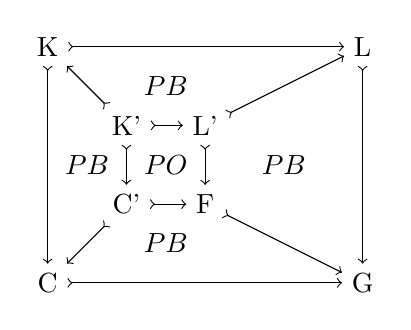
\begin{tikzpicture}
                \node (k) at (0,0) {K};
                \node (r) at (4,0) {L};
                \node (c) at (0,-3) {C};
                \node (h) at (4,-3) {G};
                \draw[<-<]  (r) -- (k) node [midway,above] {};
                \draw[>->] (c) -- (h) node [midway, below] {};
                \draw[>->] (r) -- (h) node[midway, left] {};
                \draw[>->] (k) -- (c) node[midway, left] {};
                \node (k') at (1,-1) {K'};
                \node (r') at (2,-1) {L'};
                \node (c') at (1,-2) {C'};
                \node () at (1.5,-1.5) {$PO$};
                \node () at (3,-1.5) {$PB$};
                \node () at (1.5,-2.5) {$PB$};
                \node () at (1.5,-0.5) {$PB$};
                \node () at (0.5,-1.5) {$PB$};
                \node (x) at (2,-2) {F};
                \draw [>->] (c') -- (x);
                \draw [>->] (r') -- (x);
                \draw [>->] (k') -- (r');
                \draw [>->] (k') -- (c');
                \draw [>->] (c') -- (c);
                \draw[>->] (r') -- (r);
                \draw[>->] (x) -- (h) node[midway,right] {};
                \draw[>->] (k') -- (k) ;
            \end{tikzpicture}
        \end{center} 

    There is a unique monomorphism $h_{XC'} \mathop{\colon} X \rightarrowtail C'$ 
    such that $h_{XC'} \mathop{\star} h_{C'C} \mathop{=} h_{XC}$ and $h_{XC'} \mathop{\star} h_{C'F} \mathop{=} h_{XF}$,
    because we have $h_{XF} \mathop{\star} h_{FG} \mathop{=} h_{XG}$, $h_{XC} \mathop{\star} h_{CG} \mathop{=} h_{XG}$ and $C'CGF$ is a pullback.


    Thus, we have the following commutative diagram:
    \begin{center}
        \resizebox{0.5\textwidth}{!}{
            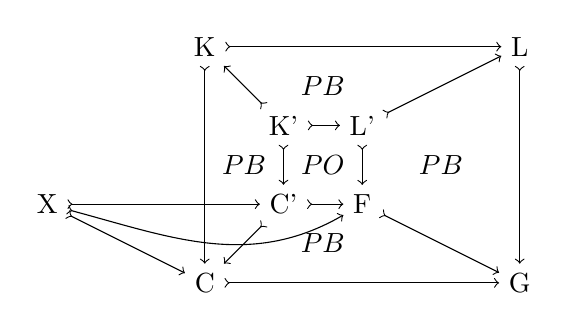
\begin{tikzpicture}
                \node (k) at (0,0) {K};
                \node (r) at (4,0) {L};
                \node (c) at (0,-3) {C};
                \node (h) at (4,-3) {G};
                % \node (rb) at ($\scl*(1.5,-0.5)$) {$R_X$};
                % \node (h') at ($\scl*(1.5,-1.5)$) {$H'$};
                % \draw[>->]  (rb) -- (h') node [midway,above] {};
                % \draw[>->]  (c) -- (h') node [midway,above] {};
                \draw[<-<]  (r) -- (k) node [midway,above] {};
                \draw[>->] (c) -- (h) node [midway, below] {$$};
                \draw[>->] (r) -- (h) node[midway, left] {$$};
                \draw[>->] (k) -- (c) node[midway, left] {};
                % \draw[->] (rb) to (l);
                % \draw[<-<] (rb) to (k);
                \node (k') at (1,-1) {K'};
                \node (r') at (2,-1) {L'};
                \node (x') at (-2,-2) {X};
                \node (c') at (1,-2) {C'};
                \node () at (1.5,-1.5) {$PO$};
                \node () at (3,-1.5) {$PB$};
                \node () at (1.5,-2.5) {$PB$};
                \node () at (1.5,-0.5) {$PB$};
                \node () at (0.5,-1.5) {$PB$};
                \node (x) at (2,-2) {F};
                % \draw [->] (x) -- (h') node[midway] {!};
                \draw [>->] (c') -- (x);
                \draw [>->] (x') -- (c');
                \draw [>->] (x') -- (c);
                \draw [>->] (x') edge[out=-15,in=210] (x);
                \draw [>->] (r') -- (x);
                \draw [>->] (k') -- (r');
                \draw [>->] (k') -- (c');
                \draw [>->] (c') -- (c);
                % \draw [->] (r') -- (rb);
                % \draw [->] (r') -- (rb);
                % \draw [->] (h') -- (h);
                \draw[>->] (r') -- (r) node[midway,below] {};
                \draw[>->] (x) -- (h) node[midway,right] {};
                % \node (rb) at ($\scl*(\sclx*1.5,-0.5)$) {$R_X$};
                % \node (h') at ($\scl*(\sclx*1.5,-1.2)$) {$H'$};
                % \draw[>->]  (rb) -- (h') node [midway,above] {};
                % \draw[>->]  (c) -- (h') node [midway,above] {};
                % \draw[>->]  (rb) -- (h') node [midway,above] {};
                % \draw[>->] (rb) to (r);
                % \draw[<-<] (rb) to (k);
                \draw[>->] (k') -- (k) ;
            \end{tikzpicture}
        }
        \end{center} 
    
     By the $F$-non-increasing property of $\rho^{-1}$,  
     \todo{assumption: the $F$-non-increasing property of $\rho^{-1}$} 
     there is a morphism $h_{L'R} \mathop{\colon} L' \rightarrowtail R$ such that $K'L'RK$ is a pullback.
        By Lemma~\ref{lem:g_monic}, there is a unique monomorphism $h_{FH} \mathop{\colon} F \rightarrowtail H$ such that $L'FHR$ and $C'FHC$ are commutative squares.
    %      $h_{L'R} \mathop{\star} h_{RH} \mathop{=} h_{L'F} \mathop{\star} h_{FH}$ and $h_{C'F} \mathop{\star} h_{FH} \mathop{=} h_{C'C} \mathop{\star} h_{CH}$, because $K'C'FL'$ is a pushout, and 
    % \begin{flalign*}
    %      &h_{K'L'} \mathop{\star} h_{L'R} \mathop{\star} h_{RH} \\
    %     =&h_{K'K} \mathop{\star} h_{KR} \mathop{\star} h_{RH} \\
    %     =&h_{K'K} \mathop{\star} h_{KC} \mathop{\star} h_{CH} \\
    %     =&h_{K'C'} \mathop{\star} h_{C'C} \mathop{\star} h_{CH}
    % \end{flalign*} 

    Thus, we have the following commutative diagram:
    \begin{center}
            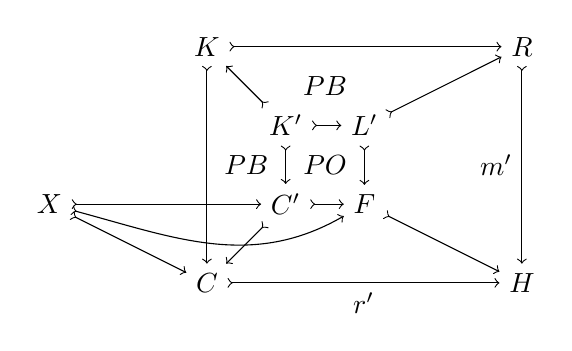
\begin{tikzpicture}
                \node (k) at (0,0) {$K$};
                \node (r) at (4,0) {$R$};
                \node (c) at (0,-3) {$C$};
                \node (h) at (4,-3) {$H$};
                \draw[<-<]  (r) -- (k) node [midway,above] {};
                \draw[>->] (c) -- (h) node [midway, below] {$r'$};
                \draw[>->] (r) -- (h) node[midway, left] {$m'$};
                \draw[>->] (k) -- (c) node[midway, left] {};
                \node (k') at (1,-1) {$K'$};
                \node (r') at (2,-1) {$L'$};
                \node (x') at (-2,-2) {$X$};
                \node (c') at (1,-2) {$C'$};
                \node () at (1.5,-1.5) {$PO$};
                \node () at (1.5,-0.5) {$PB$};
                \node () at (0.5,-1.5) {$PB$};
                \node (x) at (2,-2) {$F$};
                \draw [>->] (c') -- (x);
                \draw [>->] (x') -- (c');
                \draw [>->] (x') -- (c);
                \draw [>->] (x') edge[out=-15,in=210] (x);
                \draw [>->] (r') -- (x);
                \draw [>->] (k') -- (r');
                \draw [>->] (k') -- (c');
                \draw [>->] (c') -- (c);
                \draw[>->] (r') -- (r) node[midway,below] {};
                \draw[>->] (x) -- (h) node[midway,right] {};
                \draw[>->] (k') -- (k) ;
            \end{tikzpicture}
        \end{center} 

        Finally, we have:
        \begin{flalign*}
            \phi(h_{XG}) &= h_{XC} \mathop{\star} r' \\
            &= h_{XC'} \mathop{\star} h_{C'C} \mathop{\star} r' \\
            &= (h_{XC'} \mathop{\star} h_{C'F}) \mathop{\star} h_{FH}.
        \end{flalign*} 
    \end{itemize}
    We have thus shown that $\phi$ is well defined.
    
    Proving its injectivity is straightforward. 
    Let $h_{XG}, h_{XG}' \mathop{\in} \operatorname{Mono}(\mathcal{X},G,\lnot m, l')_{\operatorname{F}}$ such that $h_{XG} \mathop{\neq} h_{XG}'$.
    There are morphisms $h_{XC}$ and $h_{XC}'$ such that 
    \begin{itemize}
        \item $h_{XG} \mathop{=} h_{XC} \mathop{\star} l'$, and 
        \item $h_{XG}' \mathop{=} h_{XC}' \mathop{\star} l'$.
    \end{itemize}
    By injectivity of $l'$, we have $h_{XC} \mathop{\neq} h_{XC}'$. Therefore, since $r'$ is injective, we have $\phi(h_{XG}) \mathop{=} h_{XC} \mathop{\star} r' \mathop{\neq} h_{XC}' \mathop{\star} r' \mathop{=} \phi(h_{XG}')$.
\end{proof} 

\noindent
\begin*{\textbf{Lemma~\ref{antipattern:lem:xglnotmlnotlp_xhlnotmrnotrp}}}
        let \( \rho \mathop{=} (L \overset{l}{\leftarrowtail} K \overset{r}{\rightarrowtail} R) \) be a rule, and let $\mathcal{X}=(X,\mathcal{C})$ be a ruler-graph. Suppose that $\rho$ and $\rho^{-1}$ are $X$-non-increasing. For the DPO diagram:
        \begin{center}
        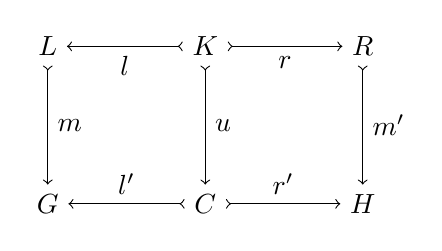
\begin{tikzpicture}
            % [node distance=15mm]
            \node (I) at (0,0) {$K$};
            \node (L) at (-2,0) {$L$};
            \node (R) at (2,0) {$R$};
            \node (G) at (-2,-2) {$G$};
            \node (C) at (0,-2) {$C$};
            \node (H) at (2,-2) {$H$}; 
            \draw [>->] (I) to  node [midway,below] {$l$} (L);
            \draw [>->] (I) to  node [midway,below] {$r$} (R);
            \draw [>->] (L) to node [midway,right] {$m$} (G);
            \draw [>->] (I) to  node [midway,right] {$u$} (C); 
            \draw [>->] (R) to  node [midway,right] {$m'$} (H);
            \draw [>->] (C) to node [midway,above] {$l'$} (G);
            \draw [>->] (C) to node [midway,above] {$r'$} (H);
        \end{tikzpicture}
    \end{center}
    the following inequality holds:
    $$ 
        \card{\operatorname{Mono}(\mathcal{X},G,\mathop{\lnot} m, \mathop{\lnot} l')_{\operatorname{NF}}} \geq
        \card{\operatorname{Mono}(\mathcal{X},H,\mathop{\lnot} m', \mathop{\lnot} r')_{\operatorname{NF}}}.
    $$ 
\end*{}
\begin{proof} 
      \label{antipattern:proof:lem:xglnotmlnotlp_xhlnotmrnotrp}
    There are two cases to consider: $\mathcal{C} \mathop{=} \emptyset$ or $\mathcal{C} \mathop{=} \set{f:X \rightarrowtail F}$. For the first case, the inequality is equivalent to the inequality:
 $$
        \card{\operatorname{Mono}(\mathcal{X},G,\lnot m, \lnot l')} \geq
        \card{\operatorname{Mono}(\mathcal{X},H,\lnot m', \lnot r')},
    $$
     and the result follows from Lemma~\ref{subgraph_counting:lem:w_u_l_not_geq_r_not}. 
    Let us now consider the second case.
     \todo{assumption for Lemma~\ref{subgraph_counting:lem:w_u_l_not_geq_r_not}: $\rho$ is $X$-non-increasing} The following equalities and inequalities hold:
    \begin{flalign*}
        & \card{\operatorname{Mono}(\mathcal{X},G,\lnot m, \lnot l')_{\operatorname{NF}}} - 
        \card{\operatorname{Mono}(\mathcal{X},H,\lnot m', \lnot r')_{\operatorname{NF}}} 
        \\
        \mathop{=} &(\card{\operatorname{Mono}(X,G,\lnot m, \lnot l')} - \card{\operatorname{Mono}(\mathcal{X},G,\lnot m, \lnot l')_{\operatorname{F}}}) -
            \\ 
           &(\card{\operatorname{Mono}(X,H,\lnot m', \lnot r')} - \card{\operatorname{Mono}(\mathcal{X},H,\lnot m', \lnot r')_{\operatorname{F}}})
        \\
        \mathop{=} &(\card{\operatorname{Mono}(X,G,\lnot m, \lnot l')} - \card{\operatorname{Mono}(X,H,\lnot m', \lnot r')})\mathop{+}
        \\ 
        &
           (\card{\operatorname{Mono}(\mathcal{X},H,\lnot m', \lnot r')_{\operatorname{F}}} - 
           \card{\operatorname{Mono}(\mathcal{X},G,\lnot m, \lnot l')_{\operatorname{F}}})
           \\
        \mathop{\geq} & 
            \card{\operatorname{Mono}(\mathcal{X},H,\lnot m', \lnot r')_{\operatorname{F}}} 
            - 
            \card{\operatorname{Mono}(\mathcal{X},G,\lnot m, \lnot l')_{\operatorname{F}}}.
        &\text{by Lemma~\ref{subgraph_counting:lem:w_u_l_not_geq_r_not}}
    \end{flalign*}    

    % We prove this lemma by show that the function $\phi: \operatorname{Mono}(\mathcal{X},G,\lnot m, \lnot l')_{\operatorname{F}} \rightarrowtail \operatorname{Mono}(X,H,\lnot r', \lnot r')_{\operatorname{NF}}$
    % defined by $\phi(h_{XG}) \mathop{=} h_{XC} \mathop{\star} \lnot r'$ is injective where $h_{XC}:X \rightarrowtail C$ is a monomorphism such that $h_{XG} \mathop{=} h_{XC} \mathop{\star} \lnot l'$.

    We prove $\card{\operatorname{Mono}(\mathcal{X},H,\lnot m', \lnot r')_{\operatorname{F}}} \mathop{\geq} \card{\operatorname{Mono}(\mathcal{X},G,\lnot m, \lnot l')_{\operatorname{F}}}$ by showing
    that we can construct an injection $\phi \mathop{\colon}  \operatorname{Mono}(\mathcal{X},G,\lnot m, \lnot l')_{\operatorname{F}} \mathop{\to} \operatorname{Mono}(\mathcal{X},H,\lnot m', \lnot r')_{\operatorname{F}}$.

    Let $h_{XG} \mathop{\in} \operatorname{Mono}(\mathcal{X},G,\lnot m, \lnot l')_{\operatorname{F}}$. 
    By Lemma~\ref{antipattern:lem:xh_decomp}, we can construct the following commutative diagram:

    \begin{center}
            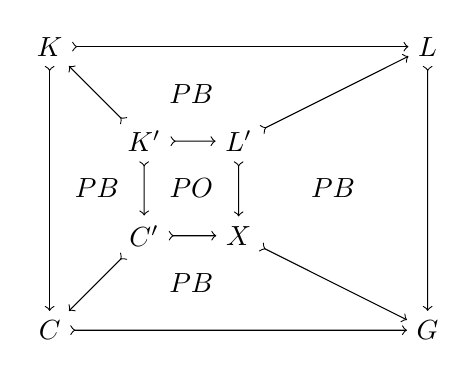
\begin{tikzpicture}[scale=1.2]
                \node (k) at (0,0) {$K$};
                \node (r) at (4,0) {$L$};
                \node (c) at (0,-3) {$C$};
                \node (h) at (4,-3) {$G$};
                \draw[<-<]  (r) -- (k) node [midway,above] {};
                \draw[>->] (c) -- (h) node [midway, below] {};
                \draw[>->] (r) -- (h) node[midway, left] {};
                \draw[>->] (k) -- (c) node[midway, left] {};
                \node (k') at (1,-1) {$K'$};
                \node (r') at (2,-1) {$L'$};
                \node (c') at (1,-2) {$C'$};
                \node () at (1.5,-1.5) {$PO$};
                \node () at (3,-1.5) {$PB$};
                \node () at (1.5,-2.5) {$PB$};
                \node () at (1.5,-0.5) {$PB$};
                \node () at (0.5,-1.5) {$PB$};
                \node (x) at (2,-2) {$X$};
                \draw [>->] (c') -- (x);
                \draw [>->] (r') -- (x);
                \draw [>->] (k') -- (r');
                \draw [>->] (k') -- (c');
                \draw [>->] (c') -- (c);
                \draw[>->] (r') -- (r);
                \draw[>->] (x) -- (h) node[midway,right] {};
                \draw[>->] (k') -- (k) ;
            \end{tikzpicture}
        \end{center} 

         \todo{assmption: $\rho^{-1}$ is $X$-non-increasing} There is a monomorphism $h_{L'R} \mathop{\colon} L' \rightarrowtail R$ because $\rho^{-1}$ is $X$-non-increasing by assumption. By Lemma~\ref{lem:g_monic}, we can construct the following commutative diagram:

        \begin{center}
                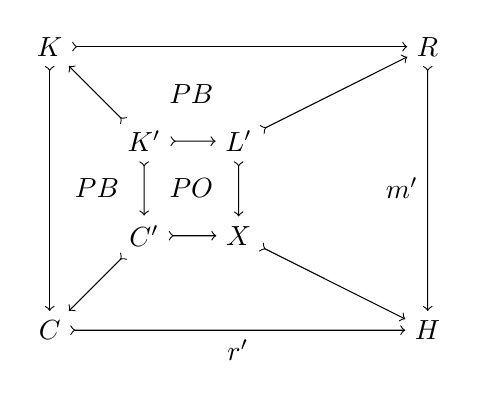
\begin{tikzpicture}[scale=1.2]
                    \node (k) at (0,0) {$K$};
                    \node (r) at (4,0) {$R$};
                    \node (c) at (0,-3) {$C$};
                    \node (h) at (4,-3) {$H$};
                    \draw[<-<]  (r) -- (k) node [midway,above] {};
                    \draw[>->] (c) -- (h) node [midway, below] {$r'$};
                    \draw[>->] (r) -- (h) node[midway, left] {$m'$};
                    \draw[>->] (k) -- (c) node[midway, left] {};
                    \node (k') at (1,-1) {$K'$};
                    \node (r') at (2,-1) {$L'$};
                    \node (c') at (1,-2) {$C'$};
                    \node () at (1.5,-1.5) {$PO$};
                    \node () at (1.5,-0.5) {$PB$};
                    \node () at (0.5,-1.5) {$PB$};
                    \node (x) at (2,-2) {$X$};
                    \draw [>->] (c') -- (x);
                    \draw [>->] (r') -- (x);
                    \draw [>->] (k') -- (r');
                    \draw [>->] (k') -- (c');
                    \draw [>->] (c') -- (c);
                    \draw[>->] (r') -- (r) node[midway,below] {};
                    \draw[>->] (x) -- (h) node[midway,right] {};
                    \draw[>->] (k') -- (k) ;
                \end{tikzpicture}
            \end{center} 

       
        We define $\phi(h_{XG}) \overset{def}{=} h_{XH}$. The function $\phi$ is injective, by Lemma~\ref{lem:h_hp_diff_g_gp_diff} \todo{ Lemma~\ref{lem:h_hp_diff_g_gp_diff} uses the assumption: $\rho$ is $X$-non-increasing}. It remains to show that $\phi$ is well defined which requires to show that $\phi(h_{XG})$ is an element in $\operatorname{Mono}(X,H,\lnot m', \lnot r')_{\operatorname{F}}$, which is equivalent to show the following three conditions:
        \begin{enumerate}
            \item $h_{XH}$ cannot be factorized by $r'$,
            \item $h_{XH}$ cannot be factorized by $m'$,
            \item there is a monomorphism $h_{FH} \mathop{\colon} F \rightarrowtail H$ such that $h_{XH} \mathop{=} f \mathop{\star} h_{FH}$.
            % $h_{XH}$ can be decomposed as $x \mathop{\star} y$ where $x$ is a monomorphism from $X$ to $F$ and $y$ is a monomorphism from $F$ to $H$.
        \end{enumerate}

        By Proposition~\ref{prop:graph_adhesive}, $KCHR$ is a VK-square. Therefore, we have the following commutative diagram:

        \begin{center}
                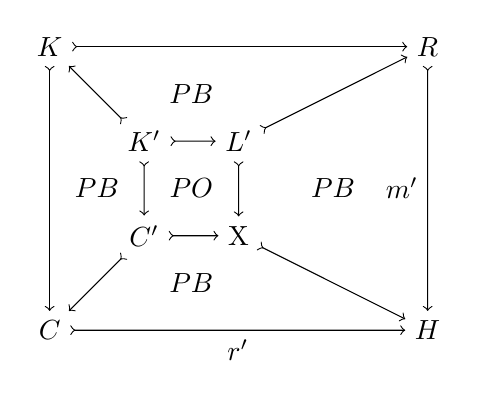
\begin{tikzpicture}[scale=1.2]
                    \node (k) at (0,0) {$K$};
                    \node (r) at (4,0) {$R$};
                    \node (c) at (0,-3) {$C$};
                    \node (h) at (4,-3) {$H$};
                    % \node (rb) at ($\scl*(1.5,-0.5)$) {$R_X$};
                    % \node (h') at ($\scl*(1.5,-1.5)$) {$H'$};
                    % \draw[>->]  (rb) -- (h') node [midway,above] {};
                    % \draw[>->]  (c) -- (h') node [midway,above] {};
                    \draw[<-<]  (r) -- (k) node [midway,above] {};
                    \draw[>->] (c) -- (h) node [midway, below] {$r'$};
                    \draw[>->] (r) -- (h) node[midway, left] {$m'$};
                    \draw[>->] (k) -- (c) node[midway, left] {};
                    % \draw[->] (rb) to (l);
                    % \draw[<-<] (rb) to (k);
                    \node (k') at (1,-1) {$K'$};
                    \node (r') at (2,-1) {$L'$};
                    \node (c') at (1,-2) {$C'$};
                    \node () at (1.5,-1.5) {$PO$};
                    \node () at (3,-1.5) {$PB$};
                    \node () at (1.5,-2.5) {$PB$};
                    \node () at (1.5,-0.5) {$PB$};
                    \node () at (0.5,-1.5) {$PB$};
                    \node (x) at (2,-2) {X};
                    % \draw [->] (x) -- (h') node[midway] {!};
                    \draw [>->] (c') -- (x);
                    \draw [>->] (r') -- (x);
                    \draw [>->] (k') -- (r');
                    \draw [>->] (k') -- (c');
                    \draw [>->] (c') -- (c);
                    % \draw [->] (r') -- (rb);
                    % \draw [->] (r') -- (rb);
                    % \draw [->] (h') -- (h);
                    \draw[>->] (r') -- (r) node[midway,below] {};
                    \draw[>->] (x) -- (h) node[midway,right] {};
                    % \node (rb) at ($\scl*(\sclx*1.5,-0.5)$) {$R_X$};
                    % \node (h') at ($\scl*(\sclx*1.5,-1.2)$) {$H'$};
                    % \draw[>->]  (rb) -- (h') node [midway,above] {};
                    % \draw[>->]  (c) -- (h') node [midway,above] {};
                    % \draw[>->]  (rb) -- (h') node [midway,above] {};
                    % \draw[>->] (rb) to (r);
                    % \draw[<-<] (rb) to (k);
                    \draw[>->] (k') -- (k) ;
                \end{tikzpicture}
            \end{center} 

        We show that $h_{XH}$ cannot be factorized by $m'$ by contradiction.
        Assume the contrary, i.e. there is a morphism $h_{XR} \mathop{\colon} X \rightarrowtail R$ such that $h_{XH} \mathop{=} h_{XR} \mathop{\star} m'$.

        There is a unique monomorphism $h_{XL'} \mathop{\colon} X \rightarrowtail L'$ such that $Id_X \mathop{=} h_{XL'} \mathop{\star} h_{L'X}$ and $h_{XR} \mathop{=} h_{XL'} \mathop{\star} h_{L'R}$ because $L'XHR$ is a pullback and $Id_X \mathop{\star} h_{XH} \mathop{=} h_{XR} \mathop{\star} h_{RH}$.
        Thus, we have the following equalities
         \begin{flalign*}
            h_{XG} \mathop{=} &Id_X  \mathop{\star} h_{XG} 
            \\
            \mathop{=} &h_{XL'} \mathop{\star} (h_{L'X} \mathop{\star} h_{XG})
            \\
            \mathop{=} &(h_{XL'} \mathop{\star} h_{L'L}) \mathop{\star} m
        \end{flalign*}
        which contradicts the fact that $h_{XG}$ cannot be factorized by $m$ for it is an element of $\operatorname{Mono}(\mathcal{X},G,\lnot m, \lnot l')_{\operatorname{F}}$.
        
        Symmetrically, $\phi(h_{XG})$ cannot be factorized by $r'$.

        It remains to show that there is a monomorphism $h_{FH} \mathop{\colon} F \rightarrowtail H$ such that $h_{XH} \mathop{=} f \mathop{\star} h_{FH}$. 
        
        Since $h_{XG} \mathop{\in} \operatorname{Mono}(\mathcal{X},G,\lnot m, \lnot l')_{\operatorname{F}}$, there is a morphism $h_{FG} \mathop{\colon} F \rightarrowtail G$ such that 
            the following equality holds:
        \begin{flalign}
            h_{XG} \mathop{=} f \mathop{\star} h_{FG}. \label{antipattern:eq:xxxhxg}
        \end{flalign}
        Thus, we have the following commutative diagram:

        \begin{center}
                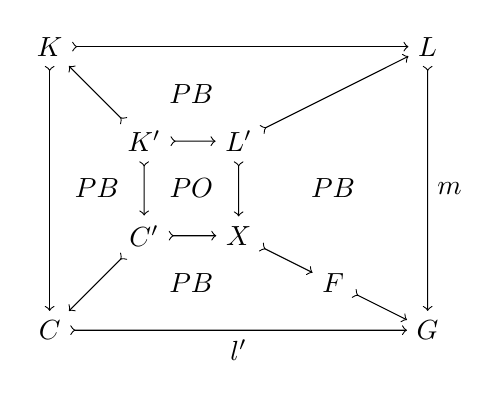
\begin{tikzpicture}[scale=1.2]
                    \node (k) at (0,0) {$K$};
                    \node (r) at (4,0) {$L$};
                    \node (c) at (0,-3) {$C$};
                    \node (x) at (2,-2) {$X$};
                    \node (h) at (4,-3) {$G$};
                    \node (f) at (3,-2.5) {$F$};
                    \draw[<-<]  (r) -- (k) node [midway,above] {};
                    \draw[>->] (c) -- (h) node [midway, below] {$l'$};
                    \draw[>->] (r) -- (h) node[midway, right] {$m$};
                    \draw[>->] (k) -- (c) node[midway, left] {};
                    \node (k') at (1,-1) {$K'$};
                    \node (r') at (2,-1) {$L'$};
                    \node (c') at (1,-2) {$C'$};
                    \node () at (1.5,-1.5) {$PO$};
                    \node () at (3,-1.5) {$PB$};
                    \node () at (1.5,-2.5) {$PB$};
                    \node () at (1.5,-0.5) {$PB$};
                    \node () at (0.5,-1.5) {$PB$};
                    \draw [>->] (c') -- (x);
                    \draw [>->] (r') -- (x);
                    \draw [>->] (k') -- (r');
                    \draw [>->] (k') -- (c');
                    \draw [>->] (c') -- (c);
                    \draw[>->] (r') -- (r) node[midway,below] {};
                    \draw[>->] (x) -- (f) node[midway,right] {};
                    \draw[>->] (f) -- (h) node[midway,right] {};
                    \draw[>->] (k') -- (k) ;
                \end{tikzpicture}
            \end{center} 


    Since we work in \textbf{Graph}, we can construct the following commutative diagram where $L''LGF$ and $C''CGF$ are pullbacks: \todo{do we need more details?}
     \begin{center}
                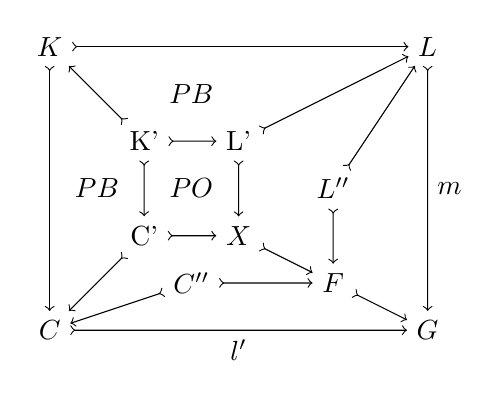
\begin{tikzpicture}[scale=1.2]
                    \node (k) at (0,0) {$K$};
                    \node (r) at (4,0) {$L$};
                    \node (c) at (0,-3) {$C$};
                    \node (x) at (2,-2) {$X$};
                    \node (h) at (4,-3) {$G$};
                    \node (f) at (3,-2.5) {$F$};
                    \draw[<-<]  (r) -- (k) node [midway,above] {};
                    \draw[>->] (c) -- (h) node [midway, below] {$l'$};
                    \draw[>->] (r) -- (h) node[midway, right] {$m$};
                    \draw[>->] (k) -- (c) node[midway, left] {};
                    \node (k') at (1,-1) {K'};
                    \node (r') at (2,-1) {L'};
                    \node (c') at (1,-2) {C'};
                    \node () at (1.5,-1.5) {$PO$};
                    \node (l'') at (3,-1.5) {$L''$};
                    \node (c'') at (1.5,-2.5) {$C''$};
                    \draw[>->] (c'') -- (c);
                    \draw[>->] (c'') --(f);
                    \draw[>->] (l'') --(f);
                    \draw[>->] (l'') --(r);
                    \node () at (1.5,-0.5) {$PB$};
                    \node () at (0.5,-1.5) {$PB$};
                    \draw [>->] (c') -- (x);
                    \draw [>->] (r') -- (x);
                    \draw [>->] (k') -- (r');
                    \draw [>->] (k') -- (c');
                    \draw [>->] (c') -- (c);
                    \draw[>->] (r') -- (r) node[midway,below] {};
                    \draw[>->] (x) -- (f) node[midway,right] {};
                    \draw[>->] (f) -- (h) node[midway,right] {};
                    \draw[>->] (k') -- (k) ;
                \end{tikzpicture}
            \end{center} 

   Since $L''LGF$ is pullback and $h_{L'X} \mathop{\star} h_{XF} \mathop{\star} h_{FG} \mathop{=} h_{L'L''} \mathop{\star} h_{L''L} \mathop{\star} h_{LG}$, by the universal property of pullback, there is a unique morphism $h_{L'L''} \mathop{\colon} L' \rightarrowtail L''$ such that 
   \begin{flalign}
         h_{L'L''} \mathop{\star} h_{L''L} &= h_{L'L} \label{antipattern:lplpplppllpl}, \\
         h_{L'X} \mathop{\star} h_{XF} & \mathop{=} h_{L'L''} \mathop{\star} h_{L''F}.
         \nonumber
        %  \label{antipattern:hlpxhxfhlplpplppf}
   \end{flalign}
   $L'L''L$ and $L'L''FX$ are commutative diagrams. Analogously, since $C''CGF$ is pullback and $C'CHFX$ is a commutative diagram, there is a unique morphism $h_{C'C''} \mathop{\colon} C' \rightarrowtail C''$ such that 
   \begin{flalign}
            h_{C'C''} \mathop{\star} h_{C''C} &= h_{C'C}, \label{antipattern:cpcppc}\\
            h_{C'C''} \mathop{\star} h_{C''F} &= h_{C'X} \mathop{\star} h_{XF}.
            \nonumber 
            %  \label{antipattern:cpxf}
   \end{flalign}
   Thus, the following diagram holds:  
    \begin{center}
                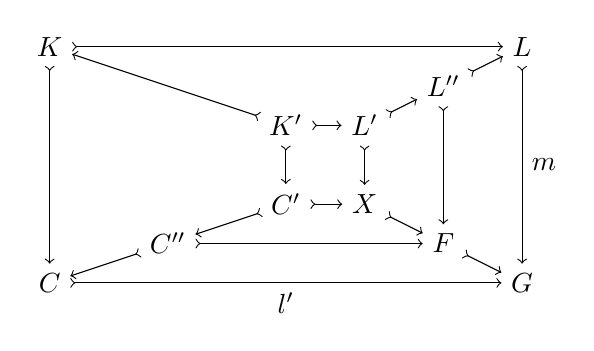
\begin{tikzpicture}
                    \node (k) at (-2,0) {$K$};
                    \node (r) at (4,0) {$L$};
                    \node (x) at (2,-2) {$X$};
                    \node (h) at (4,-3) {$G$};
                    \node (f) at (3,-2.5) {$F$};
                    \node (k') at (1,-1) {$K'$};
                    \node (r') at (2,-1) {$L'$};
                    \node (c) at (-2,-3) {$C$};
                    \node (c') at (1,-2) {$C'$};
                    \node (c'') at (-0.5,-2.5) {$C''$};
                    % \node () at (1.5,-1.5) {$PO$};
                    % \node () at (2.5,-1.5) {$PB$};
                    % \node () at (3.5,-1.5) {$PB$};
                    % \node () at (1.5,-2.3) {$PB$};
                    % \node () at (1.5,-2.8) {$PB$};
                    \node (l'') at (3,-0.5) {$L''$};
                    % \node (rb) at ($\scl*(1.5,-0.5)$) {$R_X$};
                    % \node (h') at ($\scl*(1.5,-1.5)$) {$H'$};
                    % \draw[>->]  (rb) -- (h') node [midway,above] {};
                    % \draw[>->]  (c) -- (h') node [midway,above] {};
                    \draw[<-<]  (r) -- (k) node [midway,above] {};
                    \draw[>->] (c) -- (h) node [midway, below] {$l'$};
                    \draw[>->] (r) -- (h) node[midway, right] {$m$};
                    \draw[>->] (k) -- (c) node[midway, left] {};
                    % \draw[->] (rb) to (l);
                    % \draw[<-<] (rb) to (k);
                    \draw[>->] (c'') -- (c);
                    \draw[>->] (c'') --(f);
                    \draw[>->] (l'') --(f);
                    \draw[>->] (l'') --(r);
                    % \node () at (1.5,-0.5) {$PB$};
                    % \node () at (-0.5,-1.5) {$PB$};
                    % \draw [->] (x) -- (h') node[midway] {!};
                    \draw [>->] (c') -- (x);
                    \draw [>->] (r') -- (x);
                    \draw [>->] (k') -- (r');
                    \draw [>->] (k') -- (c');
                    \draw [>->] (c') -- (c'');
                    % \draw [->] (h') -- (h);
                    \draw[>->] (r') -- (l'') node[midway,below] {};
                    \draw[>->] (x) -- (f) node[midway,right] {};
                    \draw[>->] (f) -- (h) node[midway,right] {};
                    % \node (rb) at ($\scl*(\sclx*1.5,-0.5)$) {$R_X$};
                    % \node (h') at ($\scl*(\sclx*1.5,-1.2)$) {$H'$};
                    % \draw[>->]  (rb) -- (h') node [midway,above] {};
                    % \draw[>->]  (c) -- (h') node [midway,above] {};
                    % \draw[>->]  (rb) -- (h') node [midway,above] {};
                    % \draw[>->] (rb) to (r);
                    % \draw[<-<] (rb) to (k);
                    \draw[>->] (k') -- (k) ;
                \end{tikzpicture}
            \end{center} 

   Since we work in \textbf{Graph}, we can construct $C'' \leftarrowtail K'' \rightarrowtail L''$ the pullback of $C'' \rightarrowtail F \leftarrowtail L''$, and the following commutative diagram holds:
    \begin{center}
                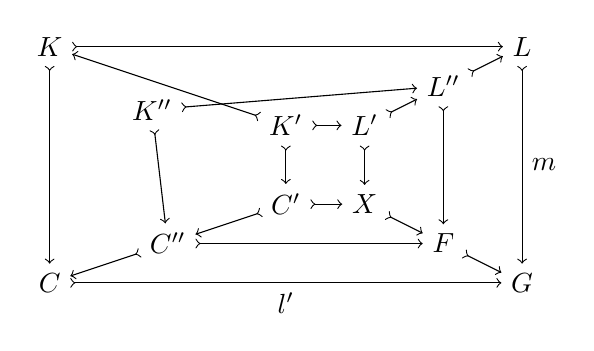
\begin{tikzpicture}
                    \node (k) at (-2,0) {$K$};
                    \node (r) at (4,0) {$L$};
                    \node (x) at (2,-2) {$X$};
                    \node (h) at (4,-3) {$G$};
                    \node (f) at (3,-2.5) {$F$};
                    \node (k') at (1,-1) {$K'$};
                    \node (r') at (2,-1) {$L'$};
                    \node (c) at (-2,-3) {$C$};
                    \node (c') at (1,-2) {$C'$};
                    \node (c'') at (-0.5,-2.5) {$C''$};
                    \node (k'') at (-0.7,-0.8) {$K''$};
                    % \node () at (1.5,-1.5) {$PO$};
                    % \node () at (2.5,-1.5) {$PB$};
                    % \node () at (3.5,-1.5) {$PB$};
                    % \node () at (1.5,-2.3) {$PB$};
                    % \node () at (1.5,-2.8) {$PB$};
                    % \node () at (1.5,-0.5) {$PB$};
                    % \node () at (-0.5,-1.5) {$PB$};
                    \node (l'') at (3,-0.5) {$L''$};
                    % \node (rb) at ($\scl*(1.5,-0.5)$) {$R_X$};
                    % \node (h') at ($\scl*(1.5,-1.5)$) {$H'$};
                    % \draw[>->]  (rb) -- (h') node [midway,above] {};
                    % \draw[>->]  (c) -- (h') node [midway,above] {};
                    % \draw[>->] (k'') -- (k) node[midway,above] {};
                    % \draw[>->] (k') -- (k'') node[midway,above] {};
                    \draw[>->] (k'') -- (c'') node[midway,above] {};
                    \draw[>->] (k'') -- (l'') node[midway,above] {};
                    \draw[<-<]  (r) -- (k) node [midway,above] {};
                    \draw[>->] (c) -- (h) node [midway, below] {$l'$};
                    \draw[>->] (r) -- (h) node[midway, right] {$m$};
                    \draw[>->] (k) -- (c) node[midway, left] {};
                    % \draw[->] (rb) to (l);
                    % \draw[<-<] (rb) to (k);
                    \draw[>->] (c'') -- (c);
                    \draw[>->] (c'') --(f);
                    \draw[>->] (l'') --(f);
                    \draw[>->] (l'') --(r);

                    % \draw [->] (x) -- (h') node[midway] {!};
                    \draw [>->] (c') -- (x);
                    \draw [>->] (r') -- (x);
                    \draw [>->] (k') -- (r');
                    \draw [>->] (k') -- (c');
                    \draw [>->] (c') -- (c'');
                    % \draw [->] (h') -- (h);
                    \draw[>->] (r') -- (l'') node[midway,below] {};
                    \draw[>->] (x) -- (f) node[midway,right] {};
                    \draw[>->] (f) -- (h) node[midway,right] {};
                    \draw[>->] (k') -- (k) ;
                \end{tikzpicture}
            \end{center} 

            Since $K''C''FL''$ is pullback and $K'C'C''FL''L'$ is a commutative diagram, by the universal property of pullback, there is a unique morphism $h_{K'K''} \mathop{\colon} K' \rightarrowtail K''$ such that $K'C'C''K''$ and $K'L'L''K''$ in the following diagram are commutative:
            \begin{center}
            \resizebox{0.5\textwidth}{!}{
                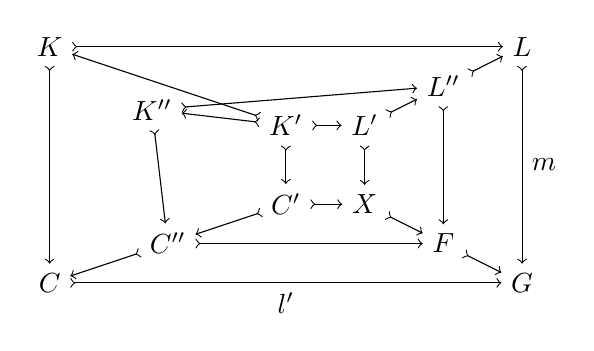
\begin{tikzpicture}
                    \node (k) at (-2,0) {$K$};
                    \node (r) at (4,0) {$L$};
                    \node (x) at (2,-2) {$X$};
                    \node (h) at (4,-3) {$G$};
                    \node (f) at (3,-2.5) {$F$};
                    \node (k') at (1,-1) {$K'$};
                    \node (r') at (2,-1) {$L'$};
                    \node (c) at (-2,-3) {$C$};
                    \node (c') at (1,-2) {$C'$};
                    \node (c'') at (-0.5,-2.5) {$C''$};
                    \node (k'') at (-0.7,-0.8) {$K''$};
                    \node (l'') at (3,-0.5) {$L''$};
                    \draw[>->] (k'') -- (c'') node[midway,above] {};
                    \draw[>->] (k'') -- (l'') node[midway,above] {};
                    \draw[<-<]  (r) -- (k) node [midway,above] {};
                    \draw[>->] (c) -- (h) node [midway, below] {$l'$};
                    \draw[>->] (r) -- (h) node[midway, right] {$m$};
                    \draw[>->] (k) -- (c) node[midway, left] {};
                    \draw[>->] (k') -- (k'') node[midway, left] {};
                    \draw[>->] (c'') -- (c);
                    \draw[>->] (c'') --(f);
                    \draw[>->] (l'') --(f);
                    \draw[>->] (l'') --(r);
                    \draw [>->] (c') -- (x);
                    \draw [>->] (r') -- (x);
                    \draw [>->] (k') -- (r');
                    \draw [>->] (k') -- (c');
                    \draw [>->] (c') -- (c'');
                    \draw[>->] (r') -- (l'') node[midway,below] {};
                    \draw[>->] (x) -- (f) node[midway,right] {};
                    \draw[>->] (f) -- (h) node[midway,right] {};
                    \draw[>->] (k') -- (k) ;
                \end{tikzpicture}
            }
            \end{center} 

          Similarly, since $KCGL$ is pullback and $K''C''CGLL''$ is a commutative diagram, by the universal property of pullback, there is a unique morphisms $h_{K''K} \mathop{\colon} K'' \rightarrowtail K$ such that $K''C''CK$, $K''L''LK$ in the following diagram are commutative:
 \begin{center}
                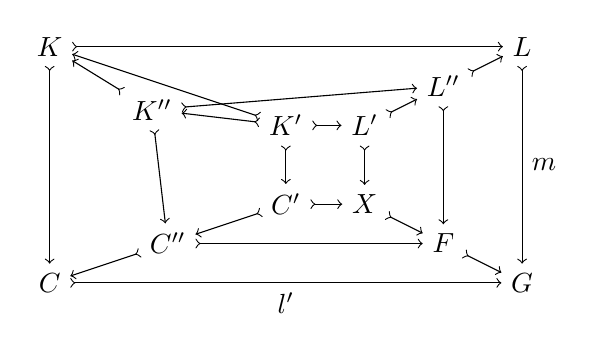
\begin{tikzpicture}
                    \node (k) at (-2,0) {$K$};
                    \node (r) at (4,0) {$L$};
                    \node (x) at (2,-2) {$X$};
                    \node (h) at (4,-3) {$G$};
                    \node (f) at (3,-2.5) {$F$};
                    \node (k') at (1,-1) {$K'$};
                    \node (r') at (2,-1) {$L'$};
                    \node (c) at (-2,-3) {$C$};
                    \node (c') at (1,-2) {$C'$};
                    \node (c'') at (-0.5,-2.5) {$C''$};
                    \node (k'') at (-0.7,-0.8) {$K''$};
                    \node (l'') at (3,-0.5) {$L''$};
                    \draw[>->] (k'') -- (k) node[midway,above] {};
                    \draw[>->] (k'') -- (c'') node[midway,above] {};
                    \draw[>->] (k'') -- (l'') node[midway,above] {};
                    \draw[<-<]  (r) -- (k) node [midway,above] {};
                    \draw[>->] (c) -- (h) node [midway, below] {$l'$};
                    \draw[>->] (r) -- (h) node[midway, right] {$m$};
                    \draw[>->] (k) -- (c) node[midway, left] {};
                    \draw[>->] (k') -- (k'') node[midway, left] {};
                    \draw[>->] (c'') -- (c);
                    \draw[>->] (c'') --(f);
                    \draw[>->] (l'') --(f);
                    \draw[>->] (l'') --(r);
                    \draw [>->] (c') -- (x);
                    \draw [>->] (r') -- (x);
                    \draw [>->] (k') -- (r');
                    \draw [>->] (k') -- (c');
                    \draw [>->] (c') -- (c'');
                    \draw[>->] (r') -- (l'') node[midway,below] {};
                    \draw[>->] (x) -- (f) node[midway,right] {};
                    \draw[>->] (f) -- (h) node[midway,right] {};
                    \draw[>->] (k') -- (k) ;
                \end{tikzpicture}
            \end{center} 

        There is a monomorphism $h_{L''R} \mathop{\colon} L'' \rightarrowtail R$ such that $K''L''RK$ is pullback, because $\rho^{-1}$ is $X$-non-increasing by assumption.\todo{$\rho^{-1}$ is $X$-non-increasing} We have, thus, the following commutative diagram:

\begin{center}
                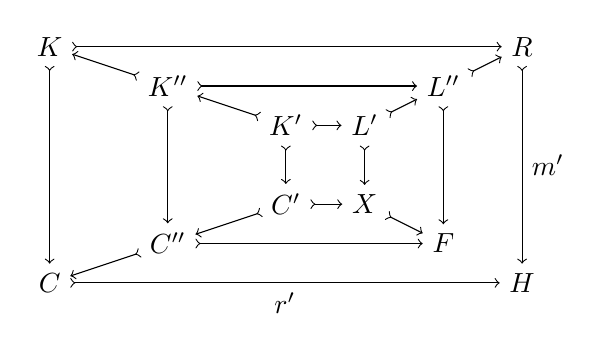
\begin{tikzpicture}
                    \node (k) at (-2,0) {$K$};
                    \node (r) at (4,0) {$R$};
                    \node (x) at (2,-2) {$X$};
                    \node (h) at (4,-3) {$H$};
                    \node (f) at (3,-2.5) {$F$};
                    \node (k') at (1,-1) {$K'$};
                    \node (r') at (2,-1) {$L'$};
                    \node (c) at (-2,-3) {$C$};
                    \node (c') at (1,-2) {$C'$};
                    \node (c'') at (-0.5,-2.5) {$C''$};
                    \node (k'') at (-0.5,-0.5) {$K''$};
                    % \node () at (1.5,-1.5) {$PO$};
                    % \node () at (2.5,-1.5) {$PB$};
                    % \node () at (3.5,-1.5) {$PB$};
                    % \node () at (1.5,-2.3) {$PB$};
                    % \node () at (1.5,-2.8) {$PB$};
                    % \node () at (1.5,-0.5) {$PB$};
                    % \node () at (-0.5,-1.5) {$PB$};
                    \node (l'') at (3,-0.5) {$L''$};
                    % \node (rb) at ($\scl*(1.5,-0.5)$) {$R_X$};
                    % \node (h') at ($\scl*(1.5,-1.5)$) {$H'$};
                    % \draw[>->]  (rb) -- (h') node [midway,above] {};
                    % \draw[>->]  (c) -- (h') node [midway,above] {};
                    % \draw[>->] (k'') -- (k) node[midway,above] {};
                    % \draw[>->] (k') -- (k'') node[midway,above] {};
                    \draw[>->] (k'') -- (c'') node[midway,above] {};
                    \draw[>->] (k'') -- (l'') node[midway,above] {};
                    \draw[<-<]  (r) -- (k) node [midway,above] {};
                    \draw[>->] (c) -- (h) node [midway, below] {$r'$};
                    \draw[>->] (r) -- (h) node[midway, right] {$m'$};
                    \draw[>->] (k) -- (c) node[midway, left] {};
                    \draw[>->] (k') -- (k'') node[midway, left] {};
                    \draw[>->] (k'') -- (k) node[midway, left] {};
                    % \draw[->] (rb) to (l);
                    % \draw[<-<] (rb) to (k);
                    \draw[>->] (c'') -- (c);
                    \draw[>->] (c'') --(f);
                    \draw[>->] (l'') --(f);
                    \draw[>->] (l'') --(r);

                    % \draw [->] (x) -- (h') node[midway] {!};
                    \draw [>->] (c') -- (x);
                    \draw [>->] (r') -- (x);
                    \draw [>->] (k') -- (r');
                    \draw [>->] (k') -- (c');
                    \draw [>->] (c') -- (c'');
                    % \draw [->] (h') -- (h);
                    \draw[>->] (r') -- (l'') node[midway,below] {};
                    \draw[>->] (x) -- (f) node[midway,right] {};
                    % \draw[>->] (f) -- (h) node[midway,right] {};
                    % \node (rb) at ($\scl*(\sclx*1.5,-0.5)$) {$R_X$};
                    % \node (h') at ($\scl*(\sclx*1.5,-1.2)$) {$H'$};
                    % \draw[>->]  (rb) -- (h') node [midway,above] {};
                    % \draw[>->]  (c) -- (h') node [midway,above] {};
                    % \draw[>->]  (rb) -- (h') node [midway,above] {};
                    % \draw[>->] (rb) to (r);
                    % \draw[<-<] (rb) to (k);
                \end{tikzpicture}
            \end{center} 
            
    The square $K''C''FL''$ is pushout because it is pullback, by Proposition~\ref{prop:pb_eq_po}. Furthermore, we have 
    \begin{flalign*}
         &(h_{K''C''} \mathop{\star} h_{C''C}) \mathop{\star} h_{CH} \\
        =&(h_{K''K} \mathop{\star} h_{KC}) \mathop{\star} h_{CH} \\
        \mathop{=} &h_{K''K} \mathop{\star} (h_{KR} \mathop{\star} h_{RH}) \\
        \mathop{=} &h_{K''L''} \mathop{\star} h_{L''R} \mathop{\star} h_{RH}.
    \end{flalign*}
    Therefore, by the universal property of pushout, 
     there is a unique morphism $h_{FH}$ such that $L''FHR$ and $C''FHC$ are commutative diagrams. Thus, we have the following commutative diagram:


        \begin{center}
            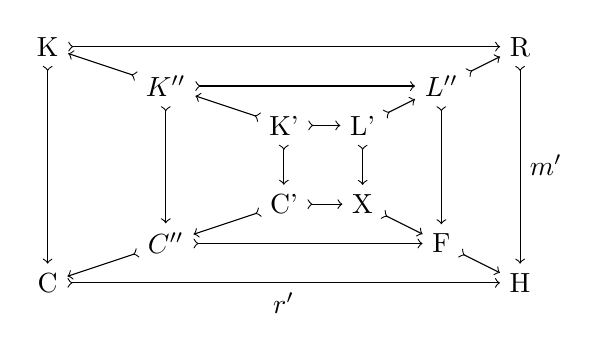
\begin{tikzpicture}
                \node (k) at (-2,0) {K};
                \node (r) at (4,0) {R};
                \node (x) at (2,-2) {X};
                \node (h) at (4,-3) {H};
                \node (f) at (3,-2.5) {F};
                \node (k') at (1,-1) {K'};
                \node (r') at (2,-1) {L'};
                \node (c) at (-2,-3) {C};
                \node (c') at (1,-2) {C'};
                \node (c'') at (-0.5,-2.5) {$C''$};
                \node (k'') at (-0.5,-0.5) {$K''$};
                \node (l'') at (3,-0.5) {$L''$};
                \draw[>->] (k'') -- (c'') node[midway,above] {};
                \draw[>->] (k'') -- (l'') node[midway,above] {};
                \draw[<-<]  (r) -- (k) node [midway,above] {};
                \draw[>->] (c) -- (h) node [midway, below] {$r'$};
                \draw[>->] (r) -- (h) node[midway, right] {$m'$};
                \draw[>->] (k) -- (c) node[midway, left] {};
                \draw[>->] (k') -- (k'') node[midway, left] {};
                \draw[>->] (k'') -- (k) node[midway, left] {};
                \draw[>->] (c'') -- (c);
                \draw[>->] (c'') --(f);
                \draw[>->] (l'') --(f);
                \draw[>->] (l'') --(r);
                \draw [>->] (c') -- (x);
                \draw [>->] (r') -- (x);
                \draw [>->] (k') -- (r');
                \draw [>->] (k') -- (c');
                \draw [>->] (c') -- (c'');
                \draw[>->] (r') -- (l'') node[midway,below] {};
                \draw[>->] (x) -- (f) node[midway,right] {};
                \draw[>->] (f) -- (h) node[midway,right] {};
            \end{tikzpicture}
        \end{center} 
    We have $h_{XH} \mathop{=} h_{XF} \mathop{\star} h_{FH}$ because $K'C'XL'$ is a pushout and $h_{XH}$ 
        is the unique morphism such that 
        \begin{flalign*}
           H_{C'X} \mathop{\star} h_{XH} &= h_{C'C} \mathop{\star} h_{CH} \\
           &=  h_{C'C''} \mathop{\star} h_{C''C} \mathop{\star} h_{CH} \hspace{2cm} \text{by~\eqref{antipattern:cpcppc}}
        \end{flalign*} and 
        \begin{flalign*}
        h_{L'X} \mathop{\star} h_{XH} &= h_{L'R} \mathop{\star} h_{RH} \\
        &= h_{L'L''} \mathop{\star} h_{L''R} \mathop{\star} h_{RH}, \hspace{2cm} \text{by~\eqref{antipattern:lplpplppllpl}}
        \end{flalign*}
         but we have 
        \begin{flalign*}
            &h_{C'X} \mathop{\star} (h_{XF} \mathop{\star} h_{FH}) 
            \\= & (h_{C'C''} \mathop{\star} h_{C''F}) \mathop{\star} h_{FH} 
            \\= & h_{C'C''} \mathop{\star} (h_{C''C} \mathop{\star} h_{CH})
        \end{flalign*}
        and 
        \begin{flalign*}
            &h_{L'X} \mathop{\star} (h_{XF} \mathop{\star} h_{FH})
            \\ \mathop{=} & (h_{L'L''} \mathop{\star} h_{L''F}) \mathop{\star} h_{FH}
            \\ \mathop{=} & h_{L'L''} \mathop{\star} (h_{L''R} \mathop{\star} h_{RH}).
        \end{flalign*}
        This concludes our proof.
\end{proof}
 
\noindent
\begin*{Theorem~\textbf{\ref{antipattern:thm:termination_grs}}}(Termination)

 Let \(\mathcal{A}\) and \(\mathcal{B}\) be sets of injective DPO rewriting rules, $\mathbb{X}$ a set of ruler-graphs, and $s_\mathbb{X}$ a weight function. If the following hold:
    \begin{enumerate}
        \item  for every $\rho \mathop{\in} \mathcal{A} \mathop{\cup} \mathcal{B}$ and for every \( \mathcal{X} \mathop{=} (X,\mathcal{C})\mathop{\in} \mathbb{X} \), 
        % the number of $X$-occurrences that are not included in any occurrences of the forbidden context $F \mathop{\in} F_x$ in a $\rho$-rewriting step is predictable,
        $\rho$ is $X$-non-increasing, and if $\mathcal{C}= \set{f:X \rightarrowtail F}$ then $\rho^{-1}$ is $X$-non-increasing and $F$-non-increasing, and
        % $\rho^{-1}$ is $F$-non-increasing if $\mathcal{X}= (X,f:X \rightarrowtail F)$ and, $\rho$ and $\rho^{-1}$ are $X$-non-increasing
        \item for every \(\rho \mathop{\in} \mathcal{A}\), we have
        % \( w_{s_\mathbb{X}}(lhs(\rho)) \mathop{>} w_{s_\mathbb{X}}(rhs(\rho)) \),
        $ \sum_{\mathcal{X} \mathop{\in} \mathbb{X}}^{}s_\mathbb{X}(\mathcal{X}) \mathop{*} 
            \Lambda(\mathcal{X},\rho) \mathop{>} 0 $, and
        \item for every \(\rho \mathop{\in} \mathcal{B}\), we have   
        % \( w_{s_\mathbb{X}}(lhs(\rho)) \mathop{\geq} w_{s_\mathbb{X}}(rhs(\rho)) \).
        $ 
            \sum_{\mathcal{X} \mathop{\in} \mathbb{X}}^{}s_\mathbb{X}(\mathcal{X}) \mathop{*} \Lambda(\mathcal{X},\rho) \mathop{\geq} 0 
        $.
    \end{enumerate}
    Then \(\mathop{\Rightarrow}_{\mathcal{A},\mathcal{M}}\) terminates relative to \(\mathop{\Rightarrow}_{\mathcal{B},\mathcal{M}}\).
\end*{}
 
\begin{proof} 
    \label{antipattern:proof:thm:termination_grs}
    
    By the assumption 1 and Lemma~\ref{antipattern:lem:w_g_geq_w_h_leq}, the following inequality holds for all rewriting steps $G \mathop{\Rightarrow}_{\rho, \mathcal{M}} H$  with $\rho \mathop{\in} \mathcal{A} \mathop{\cup} \mathcal{B}$:
      \[
        w_{s_\mathbb{X}}(G) - w_{s_\mathbb{X}}(H) 
        \mathop{\geq} 
        \sum_{\mathcal{X} \mathop{\in} \mathbb{X}}^{}s_\mathbb{X}(\mathcal{X}) * \left( 
            \card{\operatorname{Mono}(X,L)} -
            \card{\operatorname{Mono}(X,R)}
            \right).
    \]
    \noindent From the assumptions 2 and 3, we deduce 
    \begin{itemize}
        \item \( w_{s_\mathbb{X}}(G) \mathop{>} w_{s_\mathbb{X}}(H) \) for every rule \(\rho \mathop{\in} \mathcal{A}\);
        \item  \( w_{s_\mathbb{X}}(G) \mathop{\geq} w_{s_\mathbb{X}}(H) \) for every rule \(\rho \mathop{\in} \mathcal{B}\).
    \end{itemize}
    Since $w_{s_\mathbb{X}}(G) \mathop{\in} \mathbb{N}$ for all graph $G$. Every rewriting chain can only have a finite number of rewriting steps using rules from $\mathcal{A}$.
\end{proof} 